\hypertarget{group__dbprim__hash}{
\section{Hash tables}
\label{group__dbprim__hash}\index{Hash tables@{Hash tables}}
}


\subsection{Detailed Description}
Hash tables are a basic data structure used in building databases. Hash tables provide a means of storing data such that an arbitrary entry may be looked up efficiently. This library implements a hash table that may optionally grow and shrink to provide maximum efficiency. The implementation is with two kinds of caller-allocated structures--a \hyperlink{group__dbprim__hash_ga1}{hash\_\-table\_\-t} structure that describes the table and a \hyperlink{group__dbprim__hash_ga2}{hash\_\-entry\_\-t} structure for each entry in the table. The library allocates a bucket array which must be released with the \hyperlink{group__dbprim__hash_ga18}{ht\_\-free()} function when the hash table has been emptied. Additionally, the hash table may be manually resized with the \hyperlink{group__dbprim__hash_ga17}{ht\_\-resize()} function.

Entries may be added to and removed from the table using the \hyperlink{group__dbprim__hash_ga11}{ht\_\-add()} and \hyperlink{group__dbprim__hash_ga13}{ht\_\-remove()} functions. Additionally, the key on a given entry may be changed using the \hyperlink{group__dbprim__hash_ga12}{ht\_\-move()} function. Of course, any given entry may be looked up using the \hyperlink{group__dbprim__hash_ga14}{ht\_\-find()} function, and \hyperlink{group__dbprim__hash_ga15}{ht\_\-iter()} will execute a user-defined function for each entry in the hash table (in an unspecified order). The \hyperlink{group__dbprim__hash_ga16}{ht\_\-flush()} function will remove all entries from the hash table, optionally executing a user-specified clean-up function.

\subsection*{Data Structures}
\begin{CompactItemize}
\item 
struct \hyperlink{struct__hash__table__s}{\_\-hash\_\-table\_\-s}
\begin{CompactList}\small\item\em Hash table structure. \item\end{CompactList}\item 
struct \hyperlink{struct__hash__entry__s}{\_\-hash\_\-entry\_\-s}
\begin{CompactList}\small\item\em Hash table entry structure. \item\end{CompactList}\end{CompactItemize}
\subsection*{Defines}
\begin{CompactItemize}
\item 
\#define \hyperlink{group__dbprim__hash_ga21}{MAX\_\-PRIME}
\begin{CompactList}\small\item\em Largest prime. \item\end{CompactList}\item 
\#define \hyperlink{group__dbprim__hash_ga22}{HASH\_\-TABLE\_\-MAGIC}
\begin{CompactList}\small\item\em Hash table magic number. \item\end{CompactList}\item 
\#define \hyperlink{group__dbprim__hash_ga23}{HASH\_\-FLAG\_\-AUTOGROW}
\begin{CompactList}\small\item\em Flag permitting a hash table to automatically grow. \item\end{CompactList}\item 
\#define \hyperlink{group__dbprim__hash_ga24}{HASH\_\-FLAG\_\-AUTOSHRINK}
\begin{CompactList}\small\item\em Flag permitting a hash table to automatically shrink. \item\end{CompactList}\item 
\#define \hyperlink{group__dbprim__hash_ga25}{HASH\_\-FLAG\_\-MASK}
\begin{CompactList}\small\item\em Hash table flags that may be set by the user. \item\end{CompactList}\item 
\#define \hyperlink{group__dbprim__hash_ga26}{HASH\_\-TABLE\_\-INIT}(flags, func, comp, resize, extra)
\begin{CompactList}\small\item\em Hash table static initializer. \item\end{CompactList}\item 
\#define \hyperlink{group__dbprim__hash_ga27}{ht\_\-verify}(table)
\begin{CompactList}\small\item\em Hash table verification macro. \item\end{CompactList}\item 
\#define \hyperlink{group__dbprim__hash_ga28}{ht\_\-flags}(table)
\begin{CompactList}\small\item\em Hash table flags. \item\end{CompactList}\item 
\#define \hyperlink{group__dbprim__hash_ga29}{ht\_\-frozen}(table)
\begin{CompactList}\small\item\em Determine if a hash table is frozen. \item\end{CompactList}\item 
\#define \hyperlink{group__dbprim__hash_ga30}{ht\_\-modulus}(table)
\begin{CompactList}\small\item\em Hash table modulus. \item\end{CompactList}\item 
\#define \hyperlink{group__dbprim__hash_ga31}{ht\_\-count}(table)
\begin{CompactList}\small\item\em Hash table count. \item\end{CompactList}\item 
\#define \hyperlink{group__dbprim__hash_ga32}{ht\_\-func}(table)
\begin{CompactList}\small\item\em Hash table hash function. \item\end{CompactList}\item 
\#define \hyperlink{group__dbprim__hash_ga33}{ht\_\-comp}(table)
\begin{CompactList}\small\item\em Hash table comparison function. \item\end{CompactList}\item 
\#define \hyperlink{group__dbprim__hash_ga34}{ht\_\-rsize}(table)
\begin{CompactList}\small\item\em Hash table resize callback function. \item\end{CompactList}\item 
\#define \hyperlink{group__dbprim__hash_ga35}{ht\_\-extra}(table)
\begin{CompactList}\small\item\em Extra pointer data in a hash table. \item\end{CompactList}\item 
\#define \hyperlink{group__dbprim__hash_ga36}{ht\_\-size}(table)
\begin{CompactList}\small\item\em Hash table memory size. \item\end{CompactList}\item 
\#define \hyperlink{group__dbprim__hash_ga37}{HASH\_\-ENTRY\_\-MAGIC}
\begin{CompactList}\small\item\em Hash table entry magic number. \item\end{CompactList}\item 
\#define \hyperlink{group__dbprim__hash_ga38}{HASH\_\-ENTRY\_\-INIT}(value)
\begin{CompactList}\small\item\em Hash table entry static initializer. \item\end{CompactList}\item 
\#define \hyperlink{group__dbprim__hash_ga39}{he\_\-verify}(entry)
\begin{CompactList}\small\item\em Hash table entry verification macro. \item\end{CompactList}\item 
\#define \hyperlink{group__dbprim__hash_ga40}{he\_\-link}(entry)
\begin{CompactList}\small\item\em Hash table entry linked list element. \item\end{CompactList}\item 
\#define \hyperlink{group__dbprim__hash_ga41}{he\_\-flags}(entry)
\begin{CompactList}\small\item\em Hash table entry flags. \item\end{CompactList}\item 
\#define \hyperlink{group__dbprim__hash_ga42}{he\_\-table}(entry)
\begin{CompactList}\small\item\em Hash table entry table pointer. \item\end{CompactList}\item 
\#define \hyperlink{group__dbprim__hash_ga43}{he\_\-hash}(entry)
\begin{CompactList}\small\item\em Hash table entry hash value. \item\end{CompactList}\item 
\#define \hyperlink{group__dbprim__hash_ga44}{he\_\-key}(entry)
\begin{CompactList}\small\item\em Hash table entry key pointer. \item\end{CompactList}\item 
\#define \hyperlink{group__dbprim__hash_ga45}{he\_\-value}(entry)
\begin{CompactList}\small\item\em Hash table entry value pointer. \item\end{CompactList}\item 
\#define \hyperlink{group__dbprim__hash_ga46}{st\_\-rsize}(table)
\begin{CompactList}\small\item\em Sparse matrix table resize callback function. \item\end{CompactList}\item 
\#define \hyperlink{group__dbprim__hash_ga47}{\_\-hash\_\-rollover}(mod)
\begin{CompactList}\small\item\em Select hash table roll over size. \item\end{CompactList}\item 
\#define \hyperlink{group__dbprim__hash_ga48}{\_\-hash\_\-rollunder}(mod)
\begin{CompactList}\small\item\em Select hash table roll under size. \item\end{CompactList}\item 
\#define \hyperlink{group__dbprim__hash_ga49}{\_\-hash\_\-fuzz}(mod)
\begin{CompactList}\small\item\em Fuzz the initial hash table size. \item\end{CompactList}\item 
\#define \hyperlink{group__dbprim__hash_ga50}{HASH\_\-FNV\_\-OFFSET}
\begin{CompactList}\small\item\em FNV offset basis parameter. \item\end{CompactList}\item 
\#define \hyperlink{group__dbprim__hash_ga51}{HASH\_\-FNV\_\-PRIME}
\begin{CompactList}\small\item\em FNV prime parameter. \item\end{CompactList}\end{CompactItemize}
\subsection*{Typedefs}
\begin{CompactItemize}
\item 
typedef \hyperlink{struct__hash__table__s}{\_\-hash\_\-table\_\-s} \hyperlink{group__dbprim__hash_ga1}{hash\_\-table\_\-t}
\begin{CompactList}\small\item\em Hash table. \item\end{CompactList}\item 
typedef \hyperlink{struct__hash__entry__s}{\_\-hash\_\-entry\_\-s} \hyperlink{group__dbprim__hash_ga2}{hash\_\-entry\_\-t}
\begin{CompactList}\small\item\em Hash table entry. \item\end{CompactList}\item 
typedef unsigned long($\ast$ \hyperlink{group__dbprim__hash_ga3}{hash\_\-iter\_\-t} )(\hyperlink{struct__hash__table__s}{hash\_\-table\_\-t} $\ast$table, \hyperlink{struct__hash__entry__s}{hash\_\-entry\_\-t} $\ast$ent, void $\ast$extra)
\begin{CompactList}\small\item\em Hash table iteration callback. \item\end{CompactList}\item 
typedef unsigned long($\ast$ \hyperlink{group__dbprim__hash_ga4}{hash\_\-func\_\-t} )(\hyperlink{struct__hash__table__s}{hash\_\-table\_\-t} $\ast$table, \hyperlink{struct__db__key__s}{db\_\-key\_\-t} $\ast$key)
\begin{CompactList}\small\item\em Hash function callback. \item\end{CompactList}\item 
typedef unsigned long($\ast$ \hyperlink{group__dbprim__hash_ga5}{hash\_\-comp\_\-t} )(\hyperlink{struct__hash__table__s}{hash\_\-table\_\-t} $\ast$table, \hyperlink{struct__db__key__s}{db\_\-key\_\-t} $\ast$key1, \hyperlink{struct__db__key__s}{db\_\-key\_\-t} $\ast$key2)
\begin{CompactList}\small\item\em Hash table comparison callback. \item\end{CompactList}\item 
typedef unsigned long($\ast$ \hyperlink{group__dbprim__hash_ga6}{hash\_\-resize\_\-t} )(\hyperlink{struct__hash__table__s}{hash\_\-table\_\-t} $\ast$table, unsigned long new\_\-mod)
\begin{CompactList}\small\item\em Hash table resize callback. \item\end{CompactList}\end{CompactItemize}
\subsection*{Functions}
\begin{CompactItemize}
\item 
unsigned long \hyperlink{group__dbprim__hash_ga7}{hash\_\-fnv1} (\hyperlink{struct__hash__table__s}{hash\_\-table\_\-t} $\ast$table, \hyperlink{struct__db__key__s}{db\_\-key\_\-t} $\ast$key)
\begin{CompactList}\small\item\em FNV-1 hash function. \item\end{CompactList}\item 
unsigned long \hyperlink{group__dbprim__hash_ga8}{hash\_\-fnv1a} (\hyperlink{struct__hash__table__s}{hash\_\-table\_\-t} $\ast$table, \hyperlink{struct__db__key__s}{db\_\-key\_\-t} $\ast$key)
\begin{CompactList}\small\item\em FNV-1a hash function. \item\end{CompactList}\item 
unsigned long \hyperlink{group__dbprim__hash_ga9}{hash\_\-comp} (\hyperlink{struct__hash__table__s}{hash\_\-table\_\-t} $\ast$table, \hyperlink{struct__db__key__s}{db\_\-key\_\-t} $\ast$key1, \hyperlink{struct__db__key__s}{db\_\-key\_\-t} $\ast$key2)
\begin{CompactList}\small\item\em Hash comparison function. \item\end{CompactList}\item 
unsigned long \hyperlink{group__dbprim__hash_ga10}{ht\_\-init} (\hyperlink{struct__hash__table__s}{hash\_\-table\_\-t} $\ast$table, unsigned long flags, \hyperlink{group__dbprim__hash_ga4}{hash\_\-func\_\-t} func, \hyperlink{group__dbprim__hash_ga5}{hash\_\-comp\_\-t} comp, \hyperlink{group__dbprim__hash_ga6}{hash\_\-resize\_\-t} resize, void $\ast$extra, unsigned long init\_\-mod)
\begin{CompactList}\small\item\em Dynamically initialize a hash table. \item\end{CompactList}\item 
unsigned long \hyperlink{group__dbprim__hash_ga11}{ht\_\-add} (\hyperlink{struct__hash__table__s}{hash\_\-table\_\-t} $\ast$table, \hyperlink{struct__hash__entry__s}{hash\_\-entry\_\-t} $\ast$entry, \hyperlink{struct__db__key__s}{db\_\-key\_\-t} $\ast$key)
\begin{CompactList}\small\item\em Add an entry to a hash table. \item\end{CompactList}\item 
unsigned long \hyperlink{group__dbprim__hash_ga12}{ht\_\-move} (\hyperlink{struct__hash__table__s}{hash\_\-table\_\-t} $\ast$table, \hyperlink{struct__hash__entry__s}{hash\_\-entry\_\-t} $\ast$entry, \hyperlink{struct__db__key__s}{db\_\-key\_\-t} $\ast$key)
\begin{CompactList}\small\item\em Move an entry in the hash table. \item\end{CompactList}\item 
unsigned long \hyperlink{group__dbprim__hash_ga13}{ht\_\-remove} (\hyperlink{struct__hash__table__s}{hash\_\-table\_\-t} $\ast$table, \hyperlink{struct__hash__entry__s}{hash\_\-entry\_\-t} $\ast$entry)
\begin{CompactList}\small\item\em Remove an element from a hash table. \item\end{CompactList}\item 
unsigned long \hyperlink{group__dbprim__hash_ga14}{ht\_\-find} (\hyperlink{struct__hash__table__s}{hash\_\-table\_\-t} $\ast$table, \hyperlink{struct__hash__entry__s}{hash\_\-entry\_\-t} $\ast$$\ast$entry\_\-p, \hyperlink{struct__db__key__s}{db\_\-key\_\-t} $\ast$key)
\begin{CompactList}\small\item\em Find an entry in a hash table. \item\end{CompactList}\item 
unsigned long \hyperlink{group__dbprim__hash_ga15}{ht\_\-iter} (\hyperlink{struct__hash__table__s}{hash\_\-table\_\-t} $\ast$table, \hyperlink{group__dbprim__hash_ga3}{hash\_\-iter\_\-t} iter\_\-func, void $\ast$extra)
\begin{CompactList}\small\item\em Iterate over each entry in a hash table. \item\end{CompactList}\item 
unsigned long \hyperlink{group__dbprim__hash_ga16}{ht\_\-flush} (\hyperlink{struct__hash__table__s}{hash\_\-table\_\-t} $\ast$table, \hyperlink{group__dbprim__hash_ga3}{hash\_\-iter\_\-t} flush\_\-func, void $\ast$extra)
\begin{CompactList}\small\item\em Flush a hash table. \item\end{CompactList}\item 
unsigned long \hyperlink{group__dbprim__hash_ga17}{ht\_\-resize} (\hyperlink{struct__hash__table__s}{hash\_\-table\_\-t} $\ast$table, unsigned long new\_\-size)
\begin{CompactList}\small\item\em Resize a hash table. \item\end{CompactList}\item 
unsigned long \hyperlink{group__dbprim__hash_ga18}{ht\_\-free} (\hyperlink{struct__hash__table__s}{hash\_\-table\_\-t} $\ast$table)
\begin{CompactList}\small\item\em Free memory used by an empty hash table. \item\end{CompactList}\item 
unsigned long \hyperlink{group__dbprim__hash_ga19}{he\_\-init} (\hyperlink{struct__hash__entry__s}{hash\_\-entry\_\-t} $\ast$entry, void $\ast$value)
\begin{CompactList}\small\item\em Dynamically initialize a hash table entry. \item\end{CompactList}\item 
unsigned long \hyperlink{group__dbprim__hash_ga20}{\_\-hash\_\-prime} (unsigned long start)
\begin{CompactList}\small\item\em Select a prime number. \item\end{CompactList}\end{CompactItemize}
\subsection*{Variables}
\begin{CompactItemize}
\item 
static unsigned long \hyperlink{group__dbprim__hash_ga0}{primes} \mbox{[}$\,$\mbox{]}
\begin{CompactList}\small\item\em Table of primes. \item\end{CompactList}\end{CompactItemize}


\subsection{Define Documentation}
\hypertarget{group__dbprim__hash_ga49}{
\index{dbprim_hash@{dbprim\_\-hash}!_hash_fuzz@{\_\-hash\_\-fuzz}}
\index{_hash_fuzz@{\_\-hash\_\-fuzz}!dbprim_hash@{dbprim\_\-hash}}
\subsubsection[\_\-hash\_\-fuzz]{\setlength{\rightskip}{0pt plus 5cm}\#define \_\-hash\_\-fuzz(mod)}}
\label{group__dbprim__hash_ga49}


\begin{Desc}
\item[For internal use only.]
This macro is used to apply a fudge factor to a user-supplied size for the hash table, causing a slightly larger bucket to be allocated.

\begin{Desc}
\item[Parameters:]
\begin{description}
\item[\mbox{$\leftarrow$} {\em mod}]The requested table modulus.\end{description}
\end{Desc}
\begin{Desc}
\item[Returns:]The \char`\"{}fuzzed\char`\"{} size.\end{Desc}
\end{Desc}


Definition at line 107 of file dbprim\_\-int.h.

Referenced by ht\_\-add(), and ht\_\-resize().\hypertarget{group__dbprim__hash_ga47}{
\index{dbprim_hash@{dbprim\_\-hash}!_hash_rollover@{\_\-hash\_\-rollover}}
\index{_hash_rollover@{\_\-hash\_\-rollover}!dbprim_hash@{dbprim\_\-hash}}
\subsubsection[\_\-hash\_\-rollover]{\setlength{\rightskip}{0pt plus 5cm}\#define \_\-hash\_\-rollover(mod)}}
\label{group__dbprim__hash_ga47}


\begin{Desc}
\item[For internal use only.]
This macro is used to compute the \char`\"{}roll over\char`\"{} size--the size at which the hash table will be grown (assuming that the table has \hyperlink{group__dbprim__hash_ga23}{HASH\_\-FLAG\_\-AUTOGROW} set).

\begin{Desc}
\item[Parameters:]
\begin{description}
\item[\mbox{$\leftarrow$} {\em mod}]The table modulus.\end{description}
\end{Desc}
\begin{Desc}
\item[Returns:]The \char`\"{}roll over\char`\"{} size.\end{Desc}
\end{Desc}


Definition at line 79 of file dbprim\_\-int.h.

Referenced by ht\_\-init(), and ht\_\-resize().\hypertarget{group__dbprim__hash_ga48}{
\index{dbprim_hash@{dbprim\_\-hash}!_hash_rollunder@{\_\-hash\_\-rollunder}}
\index{_hash_rollunder@{\_\-hash\_\-rollunder}!dbprim_hash@{dbprim\_\-hash}}
\subsubsection[\_\-hash\_\-rollunder]{\setlength{\rightskip}{0pt plus 5cm}\#define \_\-hash\_\-rollunder(mod)}}
\label{group__dbprim__hash_ga48}


\begin{Desc}
\item[For internal use only.]
This macro is used to compute the \char`\"{}roll under\char`\"{} size--the size at which the hash table will be shrunk (assuming that the table has \hyperlink{group__dbprim__hash_ga24}{HASH\_\-FLAG\_\-AUTOSHRINK} set).

\begin{Desc}
\item[Parameters:]
\begin{description}
\item[\mbox{$\leftarrow$} {\em mod}]The table modulus.\end{description}
\end{Desc}
\begin{Desc}
\item[Returns:]The \char`\"{}roll under\char`\"{} size.\end{Desc}
\end{Desc}


Definition at line 93 of file dbprim\_\-int.h.

Referenced by ht\_\-init(), and ht\_\-resize().\hypertarget{group__dbprim__hash_ga38}{
\index{dbprim_hash@{dbprim\_\-hash}!HASH_ENTRY_INIT@{HASH\_\-ENTRY\_\-INIT}}
\index{HASH_ENTRY_INIT@{HASH\_\-ENTRY\_\-INIT}!dbprim_hash@{dbprim\_\-hash}}
\subsubsection[HASH\_\-ENTRY\_\-INIT]{\setlength{\rightskip}{0pt plus 5cm}\#define HASH\_\-ENTRY\_\-INIT(value)}}
\label{group__dbprim__hash_ga38}


This macro statically initializes a \hyperlink{group__dbprim__hash_ga2}{hash\_\-entry\_\-t}.

\begin{Desc}
\item[Parameters:]
\begin{description}
\item[\mbox{$\leftarrow$} {\em value}]A pointer to {\tt void} representing the object associated with the entry.\end{description}
\end{Desc}


Definition at line 1512 of file dbprim.h.\hypertarget{group__dbprim__hash_ga37}{
\index{dbprim_hash@{dbprim\_\-hash}!HASH_ENTRY_MAGIC@{HASH\_\-ENTRY\_\-MAGIC}}
\index{HASH_ENTRY_MAGIC@{HASH\_\-ENTRY\_\-MAGIC}!dbprim_hash@{dbprim\_\-hash}}
\subsubsection[HASH\_\-ENTRY\_\-MAGIC]{\setlength{\rightskip}{0pt plus 5cm}\#define HASH\_\-ENTRY\_\-MAGIC}}
\label{group__dbprim__hash_ga37}


\begin{Desc}
\item[For internal use only.]
This is the magic number used for the hash table entry structure.\end{Desc}


Definition at line 1502 of file dbprim.h.

Referenced by he\_\-init().\hypertarget{group__dbprim__hash_ga23}{
\index{dbprim_hash@{dbprim\_\-hash}!HASH_FLAG_AUTOGROW@{HASH\_\-FLAG\_\-AUTOGROW}}
\index{HASH_FLAG_AUTOGROW@{HASH\_\-FLAG\_\-AUTOGROW}!dbprim_hash@{dbprim\_\-hash}}
\subsubsection[HASH\_\-FLAG\_\-AUTOGROW]{\setlength{\rightskip}{0pt plus 5cm}\#define HASH\_\-FLAG\_\-AUTOGROW}}
\label{group__dbprim__hash_ga23}


If passed in to \hyperlink{group__dbprim__hash_ga26}{HASH\_\-TABLE\_\-INIT()} or \hyperlink{group__dbprim__hash_ga10}{ht\_\-init()}, allows the hash table to grow automatically.

Definition at line 1100 of file dbprim.h.

Referenced by ht\_\-add(), and ht\_\-init().\hypertarget{group__dbprim__hash_ga24}{
\index{dbprim_hash@{dbprim\_\-hash}!HASH_FLAG_AUTOSHRINK@{HASH\_\-FLAG\_\-AUTOSHRINK}}
\index{HASH_FLAG_AUTOSHRINK@{HASH\_\-FLAG\_\-AUTOSHRINK}!dbprim_hash@{dbprim\_\-hash}}
\subsubsection[HASH\_\-FLAG\_\-AUTOSHRINK]{\setlength{\rightskip}{0pt plus 5cm}\#define HASH\_\-FLAG\_\-AUTOSHRINK}}
\label{group__dbprim__hash_ga24}


If passed in to \hyperlink{group__dbprim__hash_ga26}{HASH\_\-TABLE\_\-INIT()} or \hyperlink{group__dbprim__hash_ga10}{ht\_\-init()}, allows the hash table to shrink automatically.

Definition at line 1108 of file dbprim.h.

Referenced by ht\_\-flush(), ht\_\-init(), and ht\_\-remove().\hypertarget{group__dbprim__hash_ga25}{
\index{dbprim_hash@{dbprim\_\-hash}!HASH_FLAG_MASK@{HASH\_\-FLAG\_\-MASK}}
\index{HASH_FLAG_MASK@{HASH\_\-FLAG\_\-MASK}!dbprim_hash@{dbprim\_\-hash}}
\subsubsection[HASH\_\-FLAG\_\-MASK]{\setlength{\rightskip}{0pt plus 5cm}\#define HASH\_\-FLAG\_\-MASK}}
\label{group__dbprim__hash_ga25}


This flag mask may be used to obtain flags that the hash table user may set on a hash table.

Definition at line 1116 of file dbprim.h.\hypertarget{group__dbprim__hash_ga50}{
\index{dbprim_hash@{dbprim\_\-hash}!HASH_FNV_OFFSET@{HASH\_\-FNV\_\-OFFSET}}
\index{HASH_FNV_OFFSET@{HASH\_\-FNV\_\-OFFSET}!dbprim_hash@{dbprim\_\-hash}}
\subsubsection[HASH\_\-FNV\_\-OFFSET]{\setlength{\rightskip}{0pt plus 5cm}\#define HASH\_\-FNV\_\-OFFSET}}
\label{group__dbprim__hash_ga50}


\begin{Desc}
\item[For internal use only.]
This is the 32-bit offset basis for the FNV hash algorithm. See \href{http://www.isthe.com/chongo/tech/comp/fnv/}{\tt http://www.isthe.com/chongo/tech/comp/fnv/} for more information about the FNV hash algorithm.\end{Desc}


Definition at line 117 of file dbprim\_\-int.h.

Referenced by hash\_\-fnv1(), and hash\_\-fnv1a().\hypertarget{group__dbprim__hash_ga51}{
\index{dbprim_hash@{dbprim\_\-hash}!HASH_FNV_PRIME@{HASH\_\-FNV\_\-PRIME}}
\index{HASH_FNV_PRIME@{HASH\_\-FNV\_\-PRIME}!dbprim_hash@{dbprim\_\-hash}}
\subsubsection[HASH\_\-FNV\_\-PRIME]{\setlength{\rightskip}{0pt plus 5cm}\#define HASH\_\-FNV\_\-PRIME}}
\label{group__dbprim__hash_ga51}


\begin{Desc}
\item[For internal use only.]
This is the 32-bit multiplication prime for the FNV hash algorithm. See \href{http://www.isthe.com/chongo/tech/comp/fnv/}{\tt http://www.isthe.com/chongo/tech/comp/fnv/} for more information about the FNV hash algorithm.\end{Desc}


Definition at line 127 of file dbprim\_\-int.h.

Referenced by hash\_\-fnv1(), and hash\_\-fnv1a().\hypertarget{group__dbprim__hash_ga26}{
\index{dbprim_hash@{dbprim\_\-hash}!HASH_TABLE_INIT@{HASH\_\-TABLE\_\-INIT}}
\index{HASH_TABLE_INIT@{HASH\_\-TABLE\_\-INIT}!dbprim_hash@{dbprim\_\-hash}}
\subsubsection[HASH\_\-TABLE\_\-INIT]{\setlength{\rightskip}{0pt plus 5cm}\#define HASH\_\-TABLE\_\-INIT(flags, func, comp, resize, extra)}}
\label{group__dbprim__hash_ga26}


This macro statically initializes a \hyperlink{group__dbprim__hash_ga1}{hash\_\-table\_\-t}.

\begin{Desc}
\item[Parameters:]
\begin{description}
\item[\mbox{$\leftarrow$} {\em flags}]A bit-wise OR of \hyperlink{group__dbprim__hash_ga23}{HASH\_\-FLAG\_\-AUTOGROW} and \hyperlink{group__dbprim__hash_ga24}{HASH\_\-FLAG\_\-AUTOSHRINK}. If neither behavior is desired, use 0. \item[\mbox{$\leftarrow$} {\em func}]A \hyperlink{group__dbprim__hash_ga4}{hash\_\-func\_\-t} function pointer for a hash function. \item[\mbox{$\leftarrow$} {\em comp}]A \hyperlink{group__dbprim__hash_ga5}{hash\_\-comp\_\-t} function pointer for a comparison function. \item[\mbox{$\leftarrow$} {\em resize}]A \hyperlink{group__dbprim__hash_ga6}{hash\_\-resize\_\-t} function pointer for determining whether resizing is permitted and/or for notification of the resize. \item[\mbox{$\leftarrow$} {\em extra}]Extra pointer data that should be associated with the hash table.\end{description}
\end{Desc}


Definition at line 1145 of file dbprim.h.\hypertarget{group__dbprim__hash_ga22}{
\index{dbprim_hash@{dbprim\_\-hash}!HASH_TABLE_MAGIC@{HASH\_\-TABLE\_\-MAGIC}}
\index{HASH_TABLE_MAGIC@{HASH\_\-TABLE\_\-MAGIC}!dbprim_hash@{dbprim\_\-hash}}
\subsubsection[HASH\_\-TABLE\_\-MAGIC]{\setlength{\rightskip}{0pt plus 5cm}\#define HASH\_\-TABLE\_\-MAGIC}}
\label{group__dbprim__hash_ga22}


\begin{Desc}
\item[For internal use only.]
This is the magic number used for the hash table structure.\end{Desc}


Definition at line 1092 of file dbprim.h.

Referenced by ht\_\-init().\hypertarget{group__dbprim__hash_ga41}{
\index{dbprim_hash@{dbprim\_\-hash}!he_flags@{he\_\-flags}}
\index{he_flags@{he\_\-flags}!dbprim_hash@{dbprim\_\-hash}}
\subsubsection[he\_\-flags]{\setlength{\rightskip}{0pt plus 5cm}\#define he\_\-flags(entry)}}
\label{group__dbprim__hash_ga41}


This macro retrieves a set of user-defined flags associated with the entry. It may be used as an lvalue to set those flags.

\begin{Desc}
\item[Parameters:]
\begin{description}
\item[\mbox{$\leftarrow$} {\em entry}]A pointer to a \hyperlink{group__dbprim__hash_ga2}{hash\_\-entry\_\-t}.\end{description}
\end{Desc}
\begin{Desc}
\item[Returns:]An {\tt unsigned long} containing the flags associated with the entry.\end{Desc}


Definition at line 1556 of file dbprim.h.\hypertarget{group__dbprim__hash_ga43}{
\index{dbprim_hash@{dbprim\_\-hash}!he_hash@{he\_\-hash}}
\index{he_hash@{he\_\-hash}!dbprim_hash@{dbprim\_\-hash}}
\subsubsection[he\_\-hash]{\setlength{\rightskip}{0pt plus 5cm}\#define he\_\-hash(entry)}}
\label{group__dbprim__hash_ga43}


This macro retrieves the hash value of the given hash entry. If the hash table has been resized, this value may not be the same as a previous value.

\begin{Desc}
\item[Parameters:]
\begin{description}
\item[\mbox{$\leftarrow$} {\em entry}]A pointer to a \hyperlink{group__dbprim__hash_ga2}{hash\_\-entry\_\-t}.\end{description}
\end{Desc}
\begin{Desc}
\item[Returns:]An {\tt unsigned long} containing the hash code for the entry.\end{Desc}


Definition at line 1581 of file dbprim.h.\hypertarget{group__dbprim__hash_ga44}{
\index{dbprim_hash@{dbprim\_\-hash}!he_key@{he\_\-key}}
\index{he_key@{he\_\-key}!dbprim_hash@{dbprim\_\-hash}}
\subsubsection[he\_\-key]{\setlength{\rightskip}{0pt plus 5cm}\#define he\_\-key(entry)}}
\label{group__dbprim__hash_ga44}


This macro retrieves the key associated with the hash table entry.

\begin{Desc}
\item[Parameters:]
\begin{description}
\item[\mbox{$\leftarrow$} {\em entry}]A pointer to a \hyperlink{group__dbprim__hash_ga2}{hash\_\-entry\_\-t}.\end{description}
\end{Desc}
\begin{Desc}
\item[Returns:]A pointer to a \hyperlink{group__dbprim_ga0}{db\_\-key\_\-t}.\end{Desc}


Definition at line 1592 of file dbprim.h.

Referenced by ht\_\-find().\hypertarget{group__dbprim__hash_ga40}{
\index{dbprim_hash@{dbprim\_\-hash}!he_link@{he\_\-link}}
\index{he_link@{he\_\-link}!dbprim_hash@{dbprim\_\-hash}}
\subsubsection[he\_\-link]{\setlength{\rightskip}{0pt plus 5cm}\#define he\_\-link(entry)}}
\label{group__dbprim__hash_ga40}


This macro provides access to the linked list element buried in the hash table entry. It should $\ast$not$\ast$ be used on entries currently in a hash table. The purpose of this macro is to allow an object containing a hash table entry to be placed upon a free list.

\begin{Desc}
\item[Parameters:]
\begin{description}
\item[\mbox{$\leftarrow$} {\em entry}]A pointer to a \hyperlink{group__dbprim__hash_ga2}{hash\_\-entry\_\-t}.\end{description}
\end{Desc}
\begin{Desc}
\item[Returns:]A pointer to a \hyperlink{group__dbprim__link_ga1}{link\_\-elem\_\-t}.\end{Desc}


Definition at line 1543 of file dbprim.h.\hypertarget{group__dbprim__hash_ga42}{
\index{dbprim_hash@{dbprim\_\-hash}!he_table@{he\_\-table}}
\index{he_table@{he\_\-table}!dbprim_hash@{dbprim\_\-hash}}
\subsubsection[he\_\-table]{\setlength{\rightskip}{0pt plus 5cm}\#define he\_\-table(entry)}}
\label{group__dbprim__hash_ga42}


This macro retrieves a pointer to the hash table the entry is in.

\begin{Desc}
\item[Parameters:]
\begin{description}
\item[\mbox{$\leftarrow$} {\em entry}]A pointer to a \hyperlink{group__dbprim__hash_ga2}{hash\_\-entry\_\-t}.\end{description}
\end{Desc}
\begin{Desc}
\item[Returns:]A pointer to a \hyperlink{group__dbprim__hash_ga1}{hash\_\-table\_\-t}.\end{Desc}


Definition at line 1567 of file dbprim.h.\hypertarget{group__dbprim__hash_ga45}{
\index{dbprim_hash@{dbprim\_\-hash}!he_value@{he\_\-value}}
\index{he_value@{he\_\-value}!dbprim_hash@{dbprim\_\-hash}}
\subsubsection[he\_\-value]{\setlength{\rightskip}{0pt plus 5cm}\#define he\_\-value(entry)}}
\label{group__dbprim__hash_ga45}


This macro retrieves the value associated with the hash table entry. It may be treated as an lvalue to change that value. Care should be taken when using this option.

\begin{Desc}
\item[Parameters:]
\begin{description}
\item[\mbox{$\leftarrow$} {\em entry}]A pointer to a \hyperlink{group__dbprim__hash_ga2}{hash\_\-entry\_\-t}.\end{description}
\end{Desc}
\begin{Desc}
\item[Returns:]A pointer to {\tt void} representing the value associated with this entry.\end{Desc}


Definition at line 1606 of file dbprim.h.

Referenced by \_\-st\_\-flush\_\-iter(), \_\-st\_\-iter\_\-iter(), and st\_\-find().\hypertarget{group__dbprim__hash_ga39}{
\index{dbprim_hash@{dbprim\_\-hash}!he_verify@{he\_\-verify}}
\index{he_verify@{he\_\-verify}!dbprim_hash@{dbprim\_\-hash}}
\subsubsection[he\_\-verify]{\setlength{\rightskip}{0pt plus 5cm}\#define he\_\-verify(entry)}}
\label{group__dbprim__hash_ga39}


This macro verifies that a given pointer actually does point to a hash table entry.

\begin{Desc}
\item[Warning:]This macro evaluates the {\tt entry} argument twice.\end{Desc}
\begin{Desc}
\item[Parameters:]
\begin{description}
\item[\mbox{$\leftarrow$} {\em entry}]A pointer to a \hyperlink{group__dbprim__hash_ga2}{hash\_\-entry\_\-t}.\end{description}
\end{Desc}
\begin{Desc}
\item[Returns:]Boolean {\tt true} if {\tt entry} is a valid hash table entry or {\tt false} otherwise.\end{Desc}


Definition at line 1528 of file dbprim.h.

Referenced by ht\_\-add(), ht\_\-move(), and ht\_\-remove().\hypertarget{group__dbprim__hash_ga33}{
\index{dbprim_hash@{dbprim\_\-hash}!ht_comp@{ht\_\-comp}}
\index{ht_comp@{ht\_\-comp}!dbprim_hash@{dbprim\_\-hash}}
\subsubsection[ht\_\-comp]{\setlength{\rightskip}{0pt plus 5cm}\#define ht\_\-comp(table)}}
\label{group__dbprim__hash_ga33}


This macro retrieves the comparison function pointer.

\begin{Desc}
\item[Parameters:]
\begin{description}
\item[\mbox{$\leftarrow$} {\em table}]A pointer to a \hyperlink{group__dbprim__hash_ga1}{hash\_\-table\_\-t}.\end{description}
\end{Desc}
\begin{Desc}
\item[Returns:]A \hyperlink{group__dbprim__hash_ga5}{hash\_\-comp\_\-t}.\end{Desc}


Definition at line 1243 of file dbprim.h.\hypertarget{group__dbprim__hash_ga31}{
\index{dbprim_hash@{dbprim\_\-hash}!ht_count@{ht\_\-count}}
\index{ht_count@{ht\_\-count}!dbprim_hash@{dbprim\_\-hash}}
\subsubsection[ht\_\-count]{\setlength{\rightskip}{0pt plus 5cm}\#define ht\_\-count(table)}}
\label{group__dbprim__hash_ga31}


This macro retrieves the total number of items actually in the hash table.

\begin{Desc}
\item[Parameters:]
\begin{description}
\item[\mbox{$\leftarrow$} {\em table}]A pointer to a \hyperlink{group__dbprim__hash_ga1}{hash\_\-table\_\-t}.\end{description}
\end{Desc}
\begin{Desc}
\item[Returns:]An {\tt unsigned long} containing a count of the number of items in the hash table.\end{Desc}


Definition at line 1221 of file dbprim.h.\hypertarget{group__dbprim__hash_ga35}{
\index{dbprim_hash@{dbprim\_\-hash}!ht_extra@{ht\_\-extra}}
\index{ht_extra@{ht\_\-extra}!dbprim_hash@{dbprim\_\-hash}}
\subsubsection[ht\_\-extra]{\setlength{\rightskip}{0pt plus 5cm}\#define ht\_\-extra(table)}}
\label{group__dbprim__hash_ga35}


This macro retrieves the extra pointer data associated with a particular hash table.

\begin{Desc}
\item[Parameters:]
\begin{description}
\item[\mbox{$\leftarrow$} {\em table}]A pointer to a \hyperlink{group__dbprim__hash_ga1}{hash\_\-table\_\-t}.\end{description}
\end{Desc}
\begin{Desc}
\item[Returns:]A pointer to {\tt void}.\end{Desc}


Definition at line 1266 of file dbprim.h.

Referenced by \_\-smat\_\-resize().\hypertarget{group__dbprim__hash_ga28}{
\index{dbprim_hash@{dbprim\_\-hash}!ht_flags@{ht\_\-flags}}
\index{ht_flags@{ht\_\-flags}!dbprim_hash@{dbprim\_\-hash}}
\subsubsection[ht\_\-flags]{\setlength{\rightskip}{0pt plus 5cm}\#define ht\_\-flags(table)}}
\label{group__dbprim__hash_ga28}


This macro retrieves the flags associated with the hash table. Only \hyperlink{group__dbprim__hash_ga23}{HASH\_\-FLAG\_\-AUTOGROW} and \hyperlink{group__dbprim__hash_ga24}{HASH\_\-FLAG\_\-AUTOSHRINK} have any meaning to the application; all other bits are reserved for use in the library. This macro may be used as an lvalue, but care must be taken to avoid modifying the library-specific bits.

\begin{Desc}
\item[Parameters:]
\begin{description}
\item[\mbox{$\leftarrow$} {\em table}]A pointer to a \hyperlink{group__dbprim__hash_ga1}{hash\_\-table\_\-t}.\end{description}
\end{Desc}
\begin{Desc}
\item[Returns:]An {\tt unsigned long} containing the flags for the hash table.\end{Desc}


Definition at line 1179 of file dbprim.h.\hypertarget{group__dbprim__hash_ga29}{
\index{dbprim_hash@{dbprim\_\-hash}!ht_frozen@{ht\_\-frozen}}
\index{ht_frozen@{ht\_\-frozen}!dbprim_hash@{dbprim\_\-hash}}
\subsubsection[ht\_\-frozen]{\setlength{\rightskip}{0pt plus 5cm}\#define ht\_\-frozen(table)}}
\label{group__dbprim__hash_ga29}


This macro returns a non-zero value if the table is currently frozen. The hash table may be frozen if there is an iteration in progress.

\begin{Desc}
\item[Parameters:]
\begin{description}
\item[\mbox{$\leftarrow$} {\em table}]A pointer to a \hyperlink{group__dbprim__hash_ga1}{hash\_\-table\_\-t}.\end{description}
\end{Desc}
\begin{Desc}
\item[Returns:]A zero value if the table is not frozen or a non-zero value if the table is frozen.\end{Desc}


Definition at line 1193 of file dbprim.h.\hypertarget{group__dbprim__hash_ga32}{
\index{dbprim_hash@{dbprim\_\-hash}!ht_func@{ht\_\-func}}
\index{ht_func@{ht\_\-func}!dbprim_hash@{dbprim\_\-hash}}
\subsubsection[ht\_\-func]{\setlength{\rightskip}{0pt plus 5cm}\#define ht\_\-func(table)}}
\label{group__dbprim__hash_ga32}


This macro retrieves the hash function pointer.

\begin{Desc}
\item[Parameters:]
\begin{description}
\item[\mbox{$\leftarrow$} {\em table}]A pointer to a \hyperlink{group__dbprim__hash_ga1}{hash\_\-table\_\-t}.\end{description}
\end{Desc}
\begin{Desc}
\item[Returns:]A \hyperlink{group__dbprim__hash_ga4}{hash\_\-func\_\-t}.\end{Desc}


Definition at line 1232 of file dbprim.h.\hypertarget{group__dbprim__hash_ga30}{
\index{dbprim_hash@{dbprim\_\-hash}!ht_modulus@{ht\_\-modulus}}
\index{ht_modulus@{ht\_\-modulus}!dbprim_hash@{dbprim\_\-hash}}
\subsubsection[ht\_\-modulus]{\setlength{\rightskip}{0pt plus 5cm}\#define ht\_\-modulus(table)}}
\label{group__dbprim__hash_ga30}


This macro retrieves the number of buckets allocated for the hash table. An application may wish to save this value between invocations to avoid the overhead of growing the table while filling it with data.

\begin{Desc}
\item[Parameters:]
\begin{description}
\item[\mbox{$\leftarrow$} {\em table}]A pointer to a \hyperlink{group__dbprim__hash_ga1}{hash\_\-table\_\-t}.\end{description}
\end{Desc}
\begin{Desc}
\item[Returns:]An {\tt unsigned long} containing the number of buckets allocated for the hash table.\end{Desc}


Definition at line 1208 of file dbprim.h.

Referenced by ht\_\-flush(), ht\_\-init(), ht\_\-iter(), and ht\_\-resize().\hypertarget{group__dbprim__hash_ga34}{
\index{dbprim_hash@{dbprim\_\-hash}!ht_rsize@{ht\_\-rsize}}
\index{ht_rsize@{ht\_\-rsize}!dbprim_hash@{dbprim\_\-hash}}
\subsubsection[ht\_\-rsize]{\setlength{\rightskip}{0pt plus 5cm}\#define ht\_\-rsize(table)}}
\label{group__dbprim__hash_ga34}


This macro retrieves the resize callback function pointer.

\begin{Desc}
\item[Parameters:]
\begin{description}
\item[\mbox{$\leftarrow$} {\em table}]A pointer to a \hyperlink{group__dbprim__hash_ga1}{hash\_\-table\_\-t}.\end{description}
\end{Desc}
\begin{Desc}
\item[Returns:]A \hyperlink{group__dbprim__hash_ga6}{hash\_\-resize\_\-t}.\end{Desc}


Definition at line 1254 of file dbprim.h.\hypertarget{group__dbprim__hash_ga36}{
\index{dbprim_hash@{dbprim\_\-hash}!ht_size@{ht\_\-size}}
\index{ht_size@{ht\_\-size}!dbprim_hash@{dbprim\_\-hash}}
\subsubsection[ht\_\-size]{\setlength{\rightskip}{0pt plus 5cm}\#define ht\_\-size(table)}}
\label{group__dbprim__hash_ga36}


This macro returns the physical size of the bucket array allocated by the library for this hash table.

\begin{Desc}
\item[Parameters:]
\begin{description}
\item[\mbox{$\leftarrow$} {\em table}]A pointer to a \hyperlink{group__dbprim__hash_ga1}{hash\_\-table\_\-t}.\end{description}
\end{Desc}
\begin{Desc}
\item[Returns:]A {\tt size\_\-t}.\end{Desc}


Definition at line 1278 of file dbprim.h.\hypertarget{group__dbprim__hash_ga27}{
\index{dbprim_hash@{dbprim\_\-hash}!ht_verify@{ht\_\-verify}}
\index{ht_verify@{ht\_\-verify}!dbprim_hash@{dbprim\_\-hash}}
\subsubsection[ht\_\-verify]{\setlength{\rightskip}{0pt plus 5cm}\#define ht\_\-verify(table)}}
\label{group__dbprim__hash_ga27}


This macro verifies that a given pointer actually does point to a hash table.

\begin{Desc}
\item[Warning:]This macro evaluates the {\tt table} argument twice.\end{Desc}
\begin{Desc}
\item[Parameters:]
\begin{description}
\item[\mbox{$\leftarrow$} {\em table}]A pointer to a \hyperlink{group__dbprim__hash_ga1}{hash\_\-table\_\-t}.\end{description}
\end{Desc}
\begin{Desc}
\item[Returns:]Boolean {\tt true} if {\tt table} is a valid hash table or {\tt false} otherwise.\end{Desc}


Definition at line 1162 of file dbprim.h.

Referenced by ht\_\-add(), ht\_\-find(), ht\_\-flush(), ht\_\-free(), ht\_\-iter(), ht\_\-move(), ht\_\-remove(), and ht\_\-resize().\hypertarget{group__dbprim__hash_ga21}{
\index{dbprim_hash@{dbprim\_\-hash}!MAX_PRIME@{MAX\_\-PRIME}}
\index{MAX_PRIME@{MAX\_\-PRIME}!dbprim_hash@{dbprim\_\-hash}}
\subsubsection[MAX\_\-PRIME]{\setlength{\rightskip}{0pt plus 5cm}\#define MAX\_\-PRIME}}
\label{group__dbprim__hash_ga21}


\begin{Desc}
\item[For internal use only.]
This is the largest prime number that can be handled by the \hyperlink{group__dbprim__hash_ga20}{\_\-hash\_\-prime()} function.\end{Desc}


Definition at line 41 of file \_\-hash\_\-prime.c.

Referenced by \_\-hash\_\-prime().\hypertarget{group__dbprim__hash_ga46}{
\index{dbprim_hash@{dbprim\_\-hash}!st_rsize@{st\_\-rsize}}
\index{st_rsize@{st\_\-rsize}!dbprim_hash@{dbprim\_\-hash}}
\subsubsection[st\_\-rsize]{\setlength{\rightskip}{0pt plus 5cm}\#define st\_\-rsize(table)}}
\label{group__dbprim__hash_ga46}


This macro retrieves the resize callback function pointer.

\begin{Desc}
\item[Parameters:]
\begin{description}
\item[\mbox{$\leftarrow$} {\em table}]A pointer to a \hyperlink{group__dbprim__smat_ga0}{smat\_\-table\_\-t}.\end{description}
\end{Desc}
\begin{Desc}
\item[Returns:]A \hyperlink{group__dbprim__smat_ga3}{smat\_\-resize\_\-t}.\end{Desc}


Definition at line 1763 of file dbprim.h.

\subsection{Typedef Documentation}
\hypertarget{group__dbprim__hash_ga5}{
\index{dbprim_hash@{dbprim\_\-hash}!hash_comp_t@{hash\_\-comp\_\-t}}
\index{hash_comp_t@{hash\_\-comp\_\-t}!dbprim_hash@{dbprim\_\-hash}}
\subsubsection[hash\_\-comp\_\-t]{\setlength{\rightskip}{0pt plus 5cm}typedef unsigned long($\ast$ \hyperlink{group__dbprim__hash_ga5}{hash\_\-comp\_\-t})(\hyperlink{struct__hash__table__s}{hash\_\-table\_\-t} $\ast$table, \hyperlink{struct__db__key__s}{db\_\-key\_\-t} $\ast$key1, \hyperlink{struct__db__key__s}{db\_\-key\_\-t} $\ast$key2)}}
\label{group__dbprim__hash_ga5}


This function pointer references a callback used to compare entries in a hash table. It should return 0 for identical entries and non-zero otherwise. No assumptions should be made about the order in which the two keys are passed to this function.

\begin{Desc}
\item[Parameters:]
\begin{description}
\item[\mbox{$\leftarrow$} {\em table}]A pointer to a \hyperlink{group__dbprim__hash_ga1}{hash\_\-table\_\-t}. \item[\mbox{$\leftarrow$} {\em key1}]The first key being compared. \item[\mbox{$\leftarrow$} {\em key2}]The second key being compared.\end{description}
\end{Desc}
\begin{Desc}
\item[Returns:]Zero if the keys match, non-zero otherwise.\end{Desc}


Definition at line 408 of file dbprim.h.\hypertarget{group__dbprim__hash_ga2}{
\index{dbprim_hash@{dbprim\_\-hash}!hash_entry_t@{hash\_\-entry\_\-t}}
\index{hash_entry_t@{hash\_\-entry\_\-t}!dbprim_hash@{dbprim\_\-hash}}
\subsubsection[hash\_\-entry\_\-t]{\setlength{\rightskip}{0pt plus 5cm}typedef struct \hyperlink{struct__hash__entry__s}{\_\-hash\_\-entry\_\-s} \hyperlink{struct__hash__entry__s}{hash\_\-entry\_\-t}}}
\label{group__dbprim__hash_ga2}


This structure represents a single entry of a hash table.

Definition at line 284 of file dbprim.h.\hypertarget{group__dbprim__hash_ga4}{
\index{dbprim_hash@{dbprim\_\-hash}!hash_func_t@{hash\_\-func\_\-t}}
\index{hash_func_t@{hash\_\-func\_\-t}!dbprim_hash@{dbprim\_\-hash}}
\subsubsection[hash\_\-func\_\-t]{\setlength{\rightskip}{0pt plus 5cm}typedef unsigned long($\ast$ \hyperlink{group__dbprim__hash_ga4}{hash\_\-func\_\-t})(\hyperlink{struct__hash__table__s}{hash\_\-table\_\-t} $\ast$table, \hyperlink{struct__db__key__s}{db\_\-key\_\-t} $\ast$key)}}
\label{group__dbprim__hash_ga4}


This function is associated with a hash table, and is responsible for generating a hash value. The full 32-bit range of an {\tt unsigned long} should be used--do $\ast$not$\ast$ reduce the hash value by the modulus of the hash table.

\begin{Desc}
\item[Parameters:]
\begin{description}
\item[\mbox{$\leftarrow$} {\em table}]A pointer to a \hyperlink{group__dbprim__hash_ga1}{hash\_\-table\_\-t}. \item[\mbox{$\leftarrow$} {\em key}]The database key to hash.\end{description}
\end{Desc}
\begin{Desc}
\item[Returns:]A 32-bit hash value for {\tt key}.\end{Desc}


Definition at line 392 of file dbprim.h.\hypertarget{group__dbprim__hash_ga3}{
\index{dbprim_hash@{dbprim\_\-hash}!hash_iter_t@{hash\_\-iter\_\-t}}
\index{hash_iter_t@{hash\_\-iter\_\-t}!dbprim_hash@{dbprim\_\-hash}}
\subsubsection[hash\_\-iter\_\-t]{\setlength{\rightskip}{0pt plus 5cm}typedef unsigned long($\ast$ \hyperlink{group__dbprim__hash_ga3}{hash\_\-iter\_\-t})(\hyperlink{struct__hash__table__s}{hash\_\-table\_\-t} $\ast$table, \hyperlink{struct__hash__entry__s}{hash\_\-entry\_\-t} $\ast$ent, void $\ast$extra)}}
\label{group__dbprim__hash_ga3}


This function pointer references a callback used by \hyperlink{group__dbprim__hash_ga15}{ht\_\-iter()} and \hyperlink{group__dbprim__hash_ga16}{ht\_\-flush()}. It should return 0 for success. A non-zero return value will terminate the operation and will become the return value of the \hyperlink{group__dbprim__hash_ga15}{ht\_\-iter()} or \hyperlink{group__dbprim__hash_ga16}{ht\_\-flush()} call.

\begin{Desc}
\item[Parameters:]
\begin{description}
\item[\mbox{$\leftarrow$} {\em table}]A pointer to a \hyperlink{group__dbprim__hash_ga1}{hash\_\-table\_\-t}. \item[\mbox{$\leftarrow$} {\em ent}]A pointer to the \hyperlink{group__dbprim__hash_ga2}{hash\_\-entry\_\-t} being considered. \item[\mbox{$\leftarrow$} {\em extra}]A {\tt void} pointer passed to \hyperlink{group__dbprim__hash_ga15}{ht\_\-iter()} or \hyperlink{group__dbprim__hash_ga16}{ht\_\-flush()}.\end{description}
\end{Desc}
\begin{Desc}
\item[Returns:]Zero for success, or non-zero to terminate the iteration.\end{Desc}


Definition at line 376 of file dbprim.h.\hypertarget{group__dbprim__hash_ga6}{
\index{dbprim_hash@{dbprim\_\-hash}!hash_resize_t@{hash\_\-resize\_\-t}}
\index{hash_resize_t@{hash\_\-resize\_\-t}!dbprim_hash@{dbprim\_\-hash}}
\subsubsection[hash\_\-resize\_\-t]{\setlength{\rightskip}{0pt plus 5cm}typedef unsigned long($\ast$ \hyperlink{group__dbprim__hash_ga6}{hash\_\-resize\_\-t})(\hyperlink{struct__hash__table__s}{hash\_\-table\_\-t} $\ast$table, unsigned long new\_\-mod)}}
\label{group__dbprim__hash_ga6}


This function pointer references a callback that will be called with both the old and new hash table sizes whenever a hash table is resized. It should return non-zero only when the resize should be inhibited.

\begin{Desc}
\item[Parameters:]
\begin{description}
\item[\mbox{$\leftarrow$} {\em table}]A pointer to a \hyperlink{group__dbprim__hash_ga1}{hash\_\-table\_\-t}. \item[\mbox{$\leftarrow$} {\em new\_\-mod}]The new table modulus.\end{description}
\end{Desc}
\begin{Desc}
\item[Returns:]Zero to permit the table resize, non-zero otherwise.\end{Desc}


Definition at line 424 of file dbprim.h.\hypertarget{group__dbprim__hash_ga1}{
\index{dbprim_hash@{dbprim\_\-hash}!hash_table_t@{hash\_\-table\_\-t}}
\index{hash_table_t@{hash\_\-table\_\-t}!dbprim_hash@{dbprim\_\-hash}}
\subsubsection[hash\_\-table\_\-t]{\setlength{\rightskip}{0pt plus 5cm}typedef struct \hyperlink{struct__hash__table__s}{\_\-hash\_\-table\_\-s} \hyperlink{struct__hash__table__s}{hash\_\-table\_\-t}}}
\label{group__dbprim__hash_ga1}


This structure is the basis of all hash tables maintained by this library.

Definition at line 277 of file dbprim.h.

\subsection{Function Documentation}
\hypertarget{group__dbprim__hash_ga20}{
\index{dbprim_hash@{dbprim\_\-hash}!_hash_prime@{\_\-hash\_\-prime}}
\index{_hash_prime@{\_\-hash\_\-prime}!dbprim_hash@{dbprim\_\-hash}}
\subsubsection[\_\-hash\_\-prime]{\setlength{\rightskip}{0pt plus 5cm}unsigned long \_\-hash\_\-prime (unsigned long {\em start})}}
\label{group__dbprim__hash_ga20}


\begin{Desc}
\item[For internal use only.]
This function is used by the hash table system to find the first prime number larger than {\tt start}. This prime number will be used as the hash table modulus.

\begin{Desc}
\item[Parameters:]
\begin{description}
\item[\mbox{$\leftarrow$} {\em start}]The number from which to start looking for the next largest prime.\end{description}
\end{Desc}
\begin{Desc}
\item[Returns:]The first prime number larger than {\tt start}.\end{Desc}
\end{Desc}


Definition at line 781 of file \_\-hash\_\-prime.c.

References MAX\_\-PRIME, and primes.

Referenced by ht\_\-init(), and ht\_\-resize().\hypertarget{group__dbprim__hash_ga9}{
\index{dbprim_hash@{dbprim\_\-hash}!hash_comp@{hash\_\-comp}}
\index{hash_comp@{hash\_\-comp}!dbprim_hash@{dbprim\_\-hash}}
\subsubsection[hash\_\-comp]{\setlength{\rightskip}{0pt plus 5cm}unsigned long hash\_\-comp (\hyperlink{struct__hash__table__s}{hash\_\-table\_\-t} $\ast$ {\em table}, \hyperlink{struct__db__key__s}{db\_\-key\_\-t} $\ast$ {\em key1}, \hyperlink{struct__db__key__s}{db\_\-key\_\-t} $\ast$ {\em key2})}}
\label{group__dbprim__hash_ga9}


This is a hash comparison function, compatible with \hyperlink{group__dbprim__hash_ga5}{hash\_\-comp\_\-t}, based around memcmp().

\begin{Desc}
\item[Parameters:]
\begin{description}
\item[\mbox{$\leftarrow$} {\em table}]A pointer to a \hyperlink{group__dbprim__hash_ga1}{hash\_\-table\_\-t}. \item[\mbox{$\leftarrow$} {\em key1}]The first key being compared. \item[\mbox{$\leftarrow$} {\em key2}]The second key being compared.\end{description}
\end{Desc}
\begin{Desc}
\item[Returns:]Zero if the keys match, non-zero otherwise.\end{Desc}


Definition at line 36 of file hash\_\-comp.c.

References dk\_\-key, and dk\_\-len.

Referenced by st\_\-init().\hypertarget{group__dbprim__hash_ga7}{
\index{dbprim_hash@{dbprim\_\-hash}!hash_fnv1@{hash\_\-fnv1}}
\index{hash_fnv1@{hash\_\-fnv1}!dbprim_hash@{dbprim\_\-hash}}
\subsubsection[hash\_\-fnv1]{\setlength{\rightskip}{0pt plus 5cm}unsigned long hash\_\-fnv1 (\hyperlink{struct__hash__table__s}{hash\_\-table\_\-t} $\ast$ {\em table}, \hyperlink{struct__db__key__s}{db\_\-key\_\-t} $\ast$ {\em key})}}
\label{group__dbprim__hash_ga7}


This is a hash function, compatible with \hyperlink{group__dbprim__hash_ga4}{hash\_\-func\_\-t}, based around the FNV-1 hash algorithm. See \href{http://www.isthe.com/chongo/tech/comp/fnv/}{\tt http://www.isthe.com/chongo/tech/comp/fnv/} for more information about FNV-1.

\begin{Desc}
\item[Parameters:]
\begin{description}
\item[\mbox{$\leftarrow$} {\em table}]A pointer to a \hyperlink{group__dbprim__hash_ga1}{hash\_\-table\_\-t}. \item[\mbox{$\leftarrow$} {\em key}]The database key to hash.\end{description}
\end{Desc}
\begin{Desc}
\item[Returns:]A 32-bit hash value for {\tt key}.\end{Desc}


Definition at line 35 of file hash\_\-fnv1.c.

References dk\_\-key, dk\_\-len, HASH\_\-FNV\_\-OFFSET, and HASH\_\-FNV\_\-PRIME.\hypertarget{group__dbprim__hash_ga8}{
\index{dbprim_hash@{dbprim\_\-hash}!hash_fnv1a@{hash\_\-fnv1a}}
\index{hash_fnv1a@{hash\_\-fnv1a}!dbprim_hash@{dbprim\_\-hash}}
\subsubsection[hash\_\-fnv1a]{\setlength{\rightskip}{0pt plus 5cm}unsigned long hash\_\-fnv1a (\hyperlink{struct__hash__table__s}{hash\_\-table\_\-t} $\ast$ {\em table}, \hyperlink{struct__db__key__s}{db\_\-key\_\-t} $\ast$ {\em key})}}
\label{group__dbprim__hash_ga8}


This is a hash function, compatible with \hyperlink{group__dbprim__hash_ga4}{hash\_\-func\_\-t}, based around the FNV-1a hash algorithm. See \href{http://www.isthe.com/chongo/tech/comp/fnv/}{\tt http://www.isthe.com/chongo/tech/comp/fnv/} for more information about FNV-1a.

\begin{Desc}
\item[Parameters:]
\begin{description}
\item[\mbox{$\leftarrow$} {\em table}]A pointer to a \hyperlink{group__dbprim__hash_ga1}{hash\_\-table\_\-t}. \item[\mbox{$\leftarrow$} {\em key}]The database key to hash.\end{description}
\end{Desc}
\begin{Desc}
\item[Returns:]A 32-bit hash value for {\tt key}.\end{Desc}


Definition at line 35 of file hash\_\-fnv1a.c.

References dk\_\-key, dk\_\-len, HASH\_\-FNV\_\-OFFSET, and HASH\_\-FNV\_\-PRIME.

Referenced by st\_\-init().\hypertarget{group__dbprim__hash_ga19}{
\index{dbprim_hash@{dbprim\_\-hash}!he_init@{he\_\-init}}
\index{he_init@{he\_\-init}!dbprim_hash@{dbprim\_\-hash}}
\subsubsection[he\_\-init]{\setlength{\rightskip}{0pt plus 5cm}unsigned long he\_\-init (\hyperlink{struct__hash__entry__s}{hash\_\-entry\_\-t} $\ast$ {\em entry}, void $\ast$ {\em value})}}
\label{group__dbprim__hash_ga19}


This function dynamically initializes a hash table entry.

\begin{Desc}
\item[Parameters:]
\begin{description}
\item[\mbox{$\leftarrow$} {\em entry}]A pointer to a \hyperlink{group__dbprim__hash_ga2}{hash\_\-entry\_\-t} to be initialized. \item[\mbox{$\leftarrow$} {\em value}]A pointer to {\tt void} which will be the value of the hash table entry.\end{description}
\end{Desc}
\begin{Desc}
\item[Return values:]
\begin{description}
\item[{\em DB\_\-ERR\_\-BADARGS}]A {\tt NULL} pointer was passed for {\tt entry}.\end{description}
\end{Desc}


Definition at line 34 of file he\_\-init.c.

References \_\-db\_\-key\_\-s::dk\_\-key, \_\-db\_\-key\_\-s::dk\_\-len, HASH\_\-ENTRY\_\-MAGIC, \_\-hash\_\-entry\_\-s::he\_\-elem, \_\-hash\_\-entry\_\-s::he\_\-hash, \_\-hash\_\-entry\_\-s::he\_\-key, \_\-hash\_\-entry\_\-s::he\_\-magic, \_\-hash\_\-entry\_\-s::he\_\-table, \_\-hash\_\-entry\_\-s::he\_\-value, and le\_\-init().

Referenced by \_\-smat\_\-alloc().

Here is the call graph for this function:\begin{figure}[H]
\begin{center}
\leavevmode
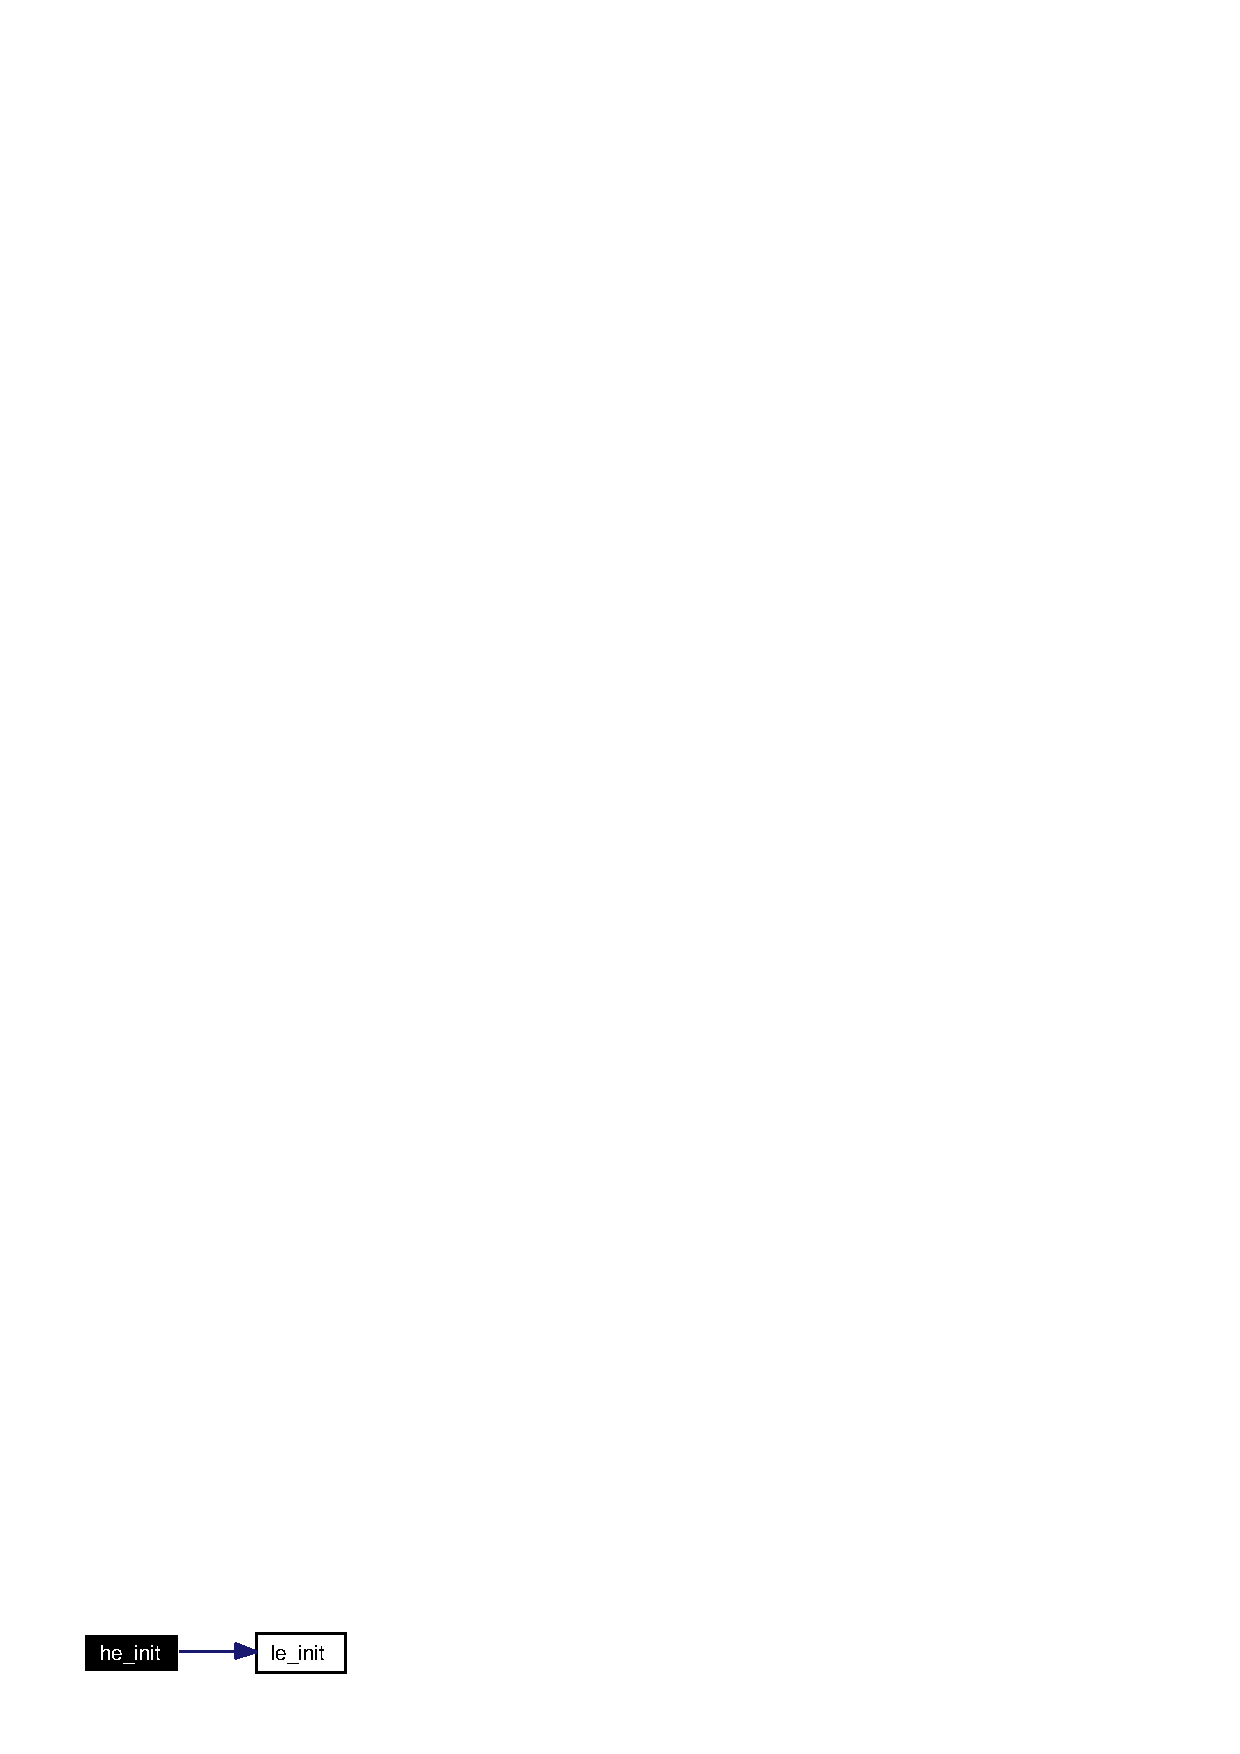
\includegraphics[width=85pt]{group__dbprim__hash_ga19_cgraph}
\end{center}
\end{figure}
\hypertarget{group__dbprim__hash_ga11}{
\index{dbprim_hash@{dbprim\_\-hash}!ht_add@{ht\_\-add}}
\index{ht_add@{ht\_\-add}!dbprim_hash@{dbprim\_\-hash}}
\subsubsection[ht\_\-add]{\setlength{\rightskip}{0pt plus 5cm}unsigned long ht\_\-add (\hyperlink{struct__hash__table__s}{hash\_\-table\_\-t} $\ast$ {\em table}, \hyperlink{struct__hash__entry__s}{hash\_\-entry\_\-t} $\ast$ {\em entry}, \hyperlink{struct__db__key__s}{db\_\-key\_\-t} $\ast$ {\em key})}}
\label{group__dbprim__hash_ga11}


This function adds an entry to a hash table.

\begin{Desc}
\item[Parameters:]
\begin{description}
\item[\mbox{$\leftarrow$} {\em table}]A pointer to a \hyperlink{group__dbprim__hash_ga1}{hash\_\-table\_\-t}. \item[\mbox{$\leftarrow$} {\em entry}]A pointer to a \hyperlink{group__dbprim__hash_ga2}{hash\_\-entry\_\-t} to be added to the table. \item[\mbox{$\leftarrow$} {\em key}]A pointer to a \hyperlink{group__dbprim_ga0}{db\_\-key\_\-t} containing the key for the entry.\end{description}
\end{Desc}
\begin{Desc}
\item[Return values:]
\begin{description}
\item[{\em DB\_\-ERR\_\-BADARGS}]An invalid argument was given. \item[{\em DB\_\-ERR\_\-BUSY}]The entry is already in a table. \item[{\em DB\_\-ERR\_\-FROZEN}]The table is currently frozen. \item[{\em DB\_\-ERR\_\-NOTABLE}]The bucket table has not been allocated and automatic growth is not enabled. \item[{\em DB\_\-ERR\_\-DUPLICATE}]The entry is a duplicate of an existing entry. \item[{\em DB\_\-ERR\_\-UNRECOVERABLE}]An unrecoverable error occurred while resizing the table.\end{description}
\end{Desc}


Definition at line 34 of file ht\_\-add.c.

References \_\-hash\_\-fuzz, HASH\_\-FLAG\_\-AUTOGROW, HASH\_\-FLAG\_\-FREEZE, \_\-hash\_\-entry\_\-s::he\_\-elem, \_\-hash\_\-entry\_\-s::he\_\-hash, \_\-hash\_\-entry\_\-s::he\_\-key, \_\-hash\_\-entry\_\-s::he\_\-table, he\_\-verify, \_\-hash\_\-table\_\-s::ht\_\-count, ht\_\-find(), \_\-hash\_\-table\_\-s::ht\_\-flags, \_\-hash\_\-table\_\-s::ht\_\-func, \_\-hash\_\-table\_\-s::ht\_\-modulus, ht\_\-resize(), \_\-hash\_\-table\_\-s::ht\_\-rollover, \_\-hash\_\-table\_\-s::ht\_\-table, ht\_\-verify, le\_\-object, LINK\_\-LOC\_\-HEAD, and ll\_\-add().

Referenced by st\_\-add().

Here is the call graph for this function:\begin{figure}[H]
\begin{center}
\leavevmode
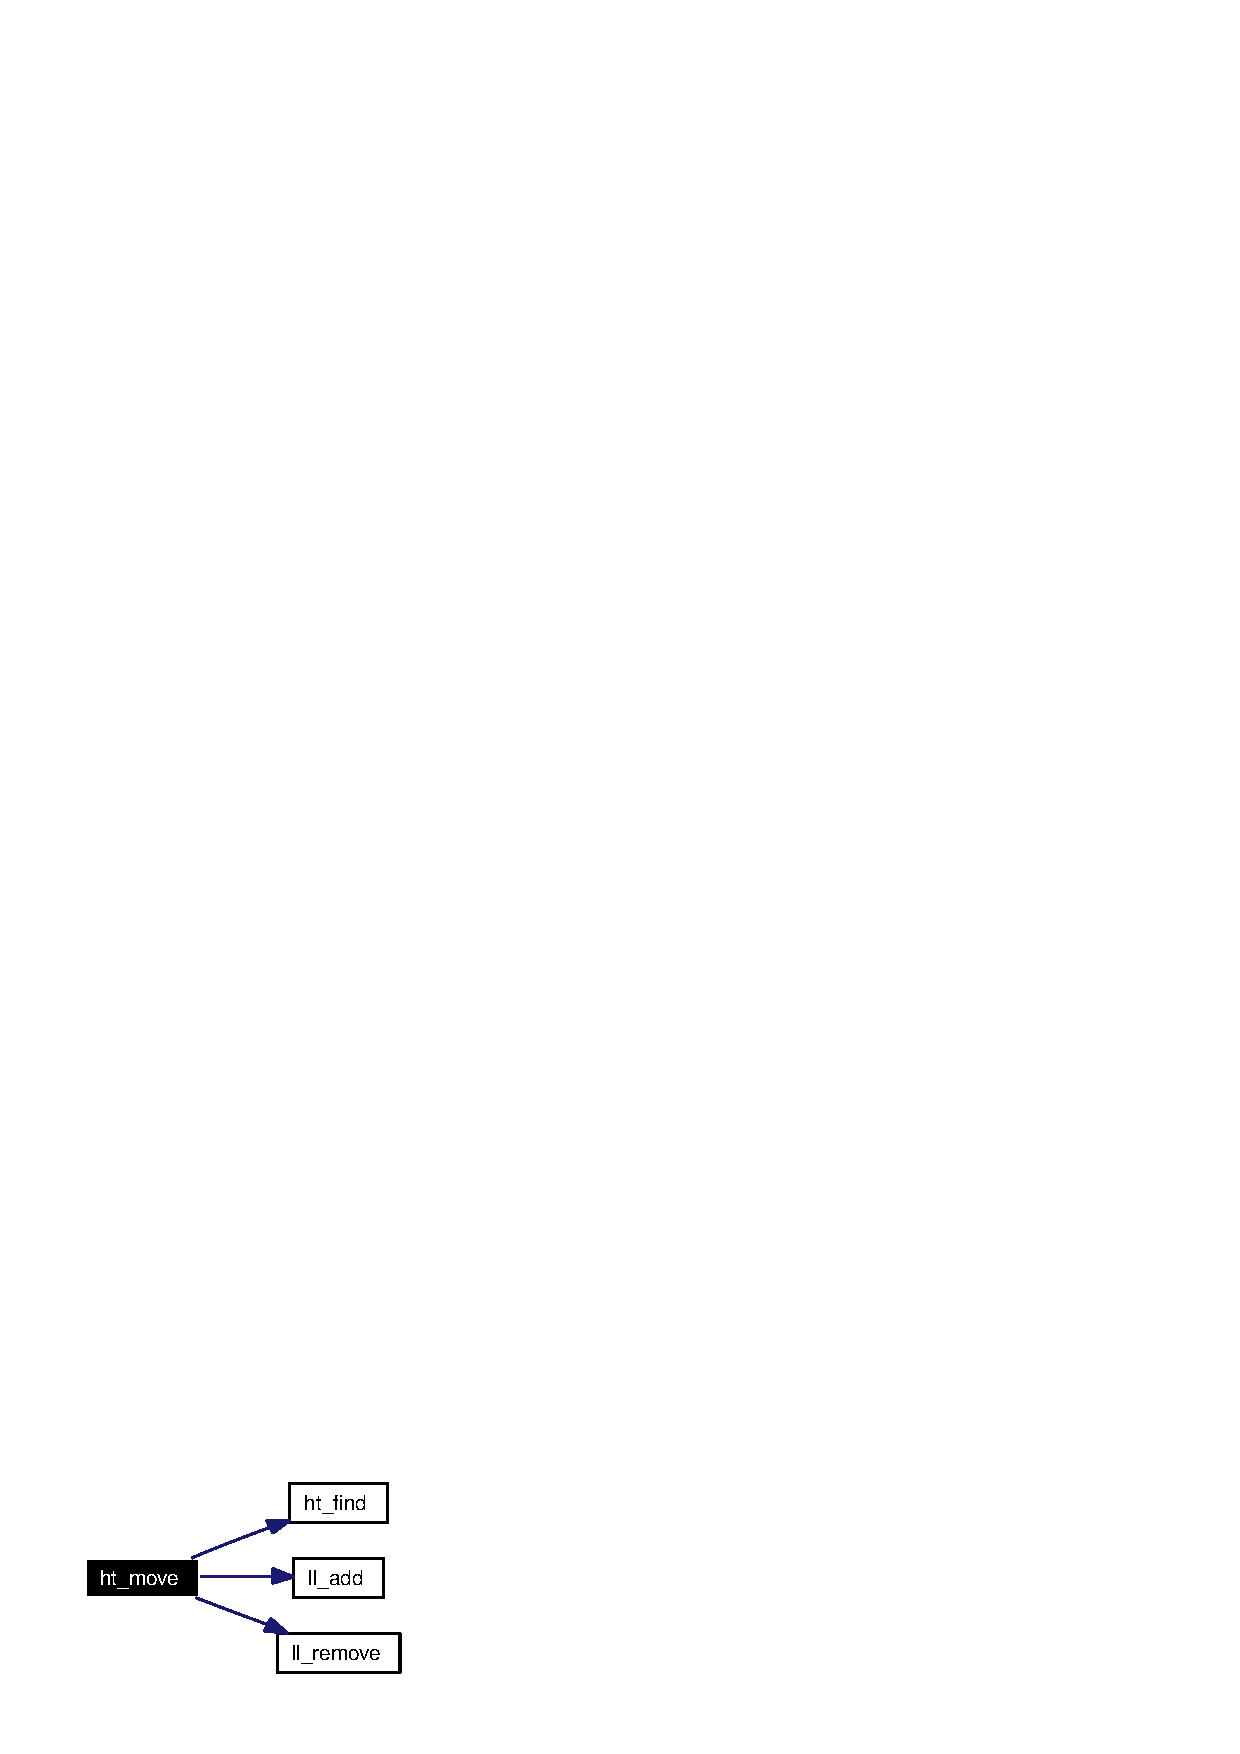
\includegraphics[width=149pt]{group__dbprim__hash_ga11_cgraph}
\end{center}
\end{figure}
\hypertarget{group__dbprim__hash_ga14}{
\index{dbprim_hash@{dbprim\_\-hash}!ht_find@{ht\_\-find}}
\index{ht_find@{ht\_\-find}!dbprim_hash@{dbprim\_\-hash}}
\subsubsection[ht\_\-find]{\setlength{\rightskip}{0pt plus 5cm}unsigned long ht\_\-find (\hyperlink{struct__hash__table__s}{hash\_\-table\_\-t} $\ast$ {\em table}, \hyperlink{struct__hash__entry__s}{hash\_\-entry\_\-t} $\ast$$\ast$ {\em entry\_\-p}, \hyperlink{struct__db__key__s}{db\_\-key\_\-t} $\ast$ {\em key})}}
\label{group__dbprim__hash_ga14}


This function looks up an entry matching the given {\tt key}.

\begin{Desc}
\item[Parameters:]
\begin{description}
\item[\mbox{$\leftarrow$} {\em table}]A pointer to a \hyperlink{group__dbprim__hash_ga1}{hash\_\-table\_\-t}. \item[\mbox{$\rightarrow$} {\em entry\_\-p}]A pointer to a pointer to a \hyperlink{group__dbprim__hash_ga2}{hash\_\-entry\_\-t}. If {\tt NULL} is passed, the lookup will be performed and an appropriate error code returned. \item[\mbox{$\leftarrow$} {\em key}]A pointer to a \hyperlink{group__dbprim_ga0}{db\_\-key\_\-t} describing the item to find.\end{description}
\end{Desc}
\begin{Desc}
\item[Return values:]
\begin{description}
\item[{\em DB\_\-ERR\_\-BADARGS}]An argument was invalid. \item[{\em DB\_\-ERR\_\-NOENTRY}]No matching entry was found.\end{description}
\end{Desc}


Definition at line 34 of file ht\_\-find.c.

References he\_\-key, \_\-hash\_\-table\_\-s::ht\_\-comp, \_\-hash\_\-table\_\-s::ht\_\-count, \_\-hash\_\-table\_\-s::ht\_\-func, \_\-hash\_\-table\_\-s::ht\_\-modulus, \_\-hash\_\-table\_\-s::ht\_\-table, ht\_\-verify, le\_\-next, le\_\-object, and ll\_\-first.

Referenced by ht\_\-add(), ht\_\-move(), and st\_\-find().\hypertarget{group__dbprim__hash_ga16}{
\index{dbprim_hash@{dbprim\_\-hash}!ht_flush@{ht\_\-flush}}
\index{ht_flush@{ht\_\-flush}!dbprim_hash@{dbprim\_\-hash}}
\subsubsection[ht\_\-flush]{\setlength{\rightskip}{0pt plus 5cm}unsigned long ht\_\-flush (\hyperlink{struct__hash__table__s}{hash\_\-table\_\-t} $\ast$ {\em table}, \hyperlink{group__dbprim__hash_ga3}{hash\_\-iter\_\-t} {\em flush\_\-func}, void $\ast$ {\em extra})}}
\label{group__dbprim__hash_ga16}


This function flushes a hash table--that is, it removes each entry from the table. If a {\tt flush\_\-func} is specified, it will be called on the entry after it has been removed from the table, and may safely call {\tt free()}.

\begin{Desc}
\item[Parameters:]
\begin{description}
\item[\mbox{$\leftarrow$} {\em table}]A pointer to a \hyperlink{group__dbprim__hash_ga1}{hash\_\-table\_\-t}. \item[\mbox{$\leftarrow$} {\em flush\_\-func}]A pointer to a callback function used to perform user-specified actions on an entry after removing it from the table. May be {\tt NULL}. See the documentation for \hyperlink{group__dbprim__hash_ga3}{hash\_\-iter\_\-t} for more information. \item[\mbox{$\leftarrow$} {\em extra}]A {\tt void} pointer that will be passed to {\tt flush\_\-func}.\end{description}
\end{Desc}
\begin{Desc}
\item[Return values:]
\begin{description}
\item[{\em DB\_\-ERR\_\-BADARGS}]An argument was invalid. \item[{\em DB\_\-ERR\_\-FROZEN}]The hash table is frozen.\end{description}
\end{Desc}


Definition at line 36 of file ht\_\-flush.c.

References HASH\_\-FLAG\_\-AUTOSHRINK, HASH\_\-FLAG\_\-FREEZE, \_\-hash\_\-table\_\-s::ht\_\-count, \_\-hash\_\-table\_\-s::ht\_\-flags, ht\_\-free(), ht\_\-modulus, ht\_\-remove(), \_\-hash\_\-table\_\-s::ht\_\-table, ht\_\-verify, le\_\-object, and ll\_\-first.

Referenced by st\_\-flush().

Here is the call graph for this function:\begin{figure}[H]
\begin{center}
\leavevmode
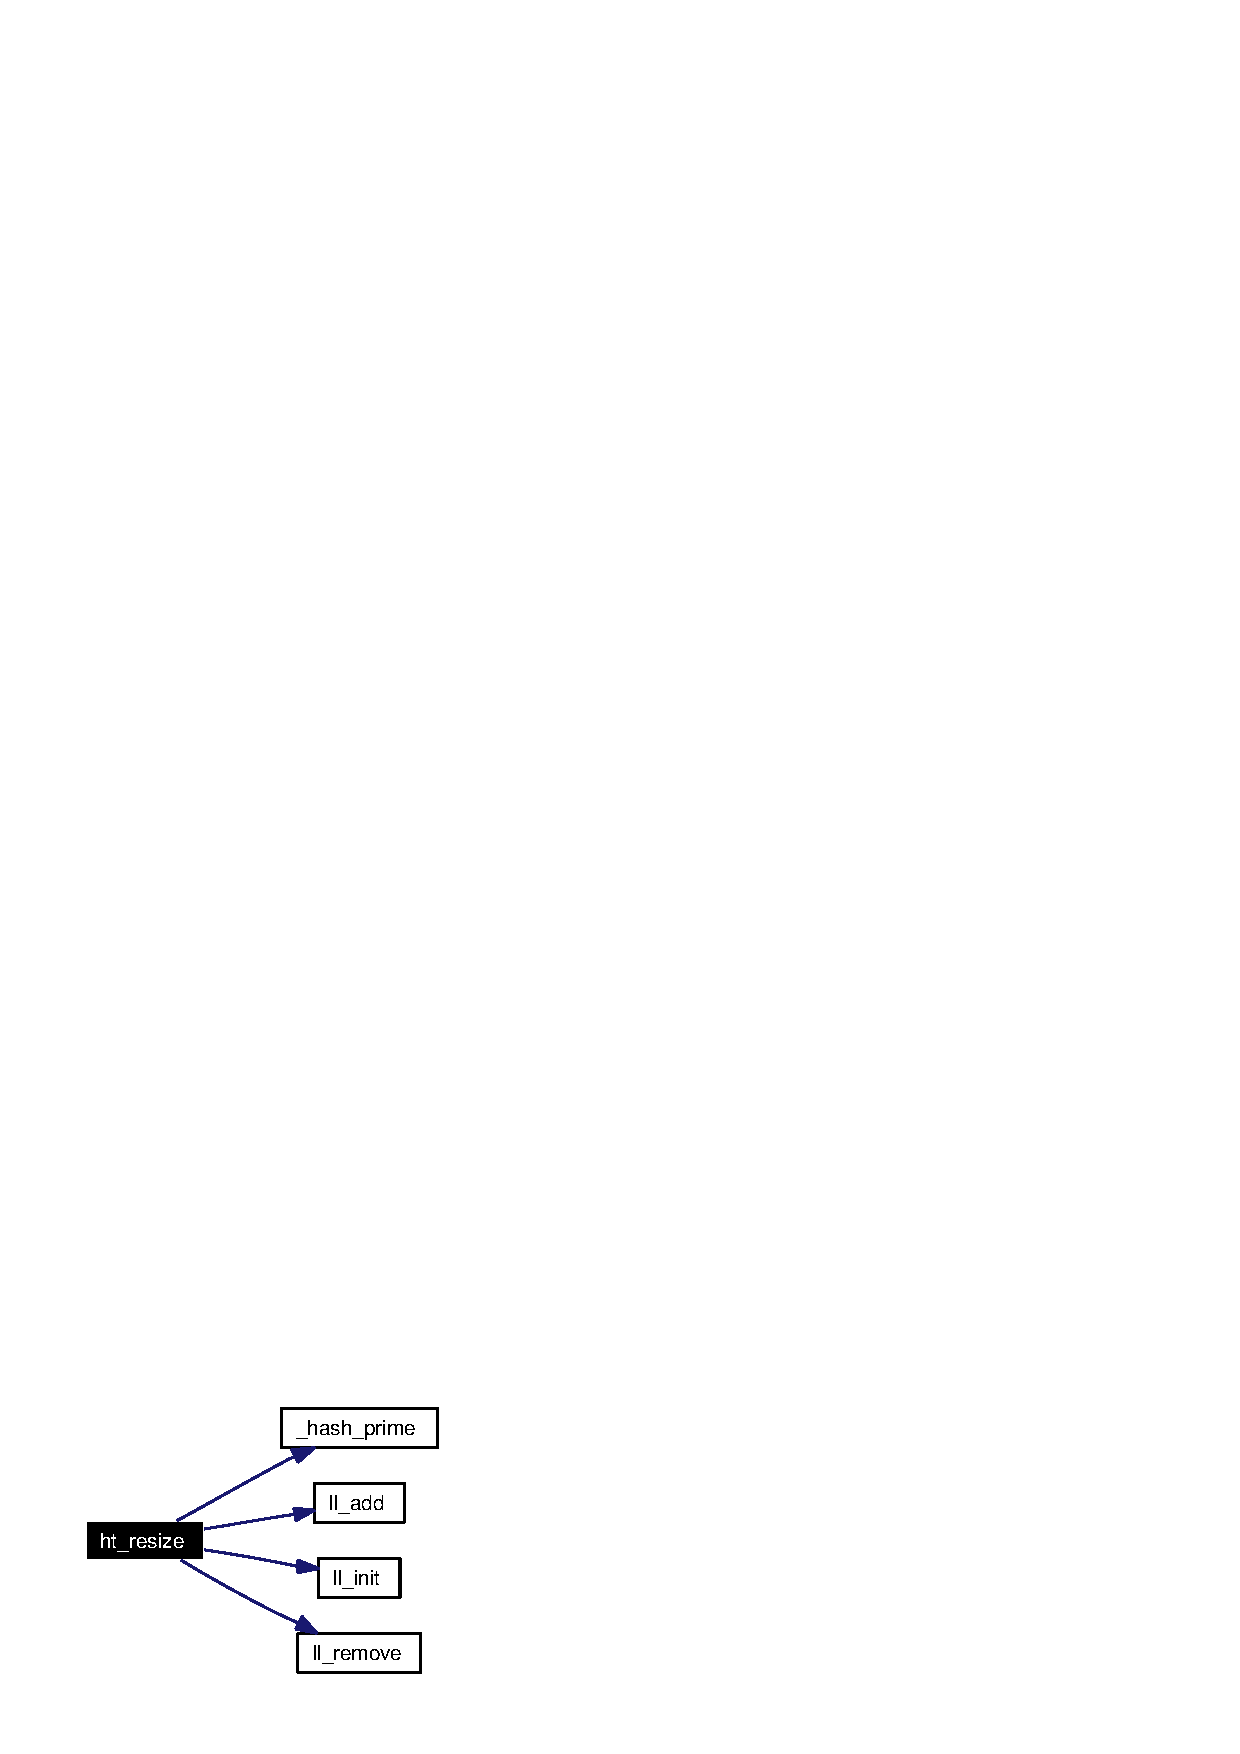
\includegraphics[width=201pt]{group__dbprim__hash_ga16_cgraph}
\end{center}
\end{figure}
\hypertarget{group__dbprim__hash_ga18}{
\index{dbprim_hash@{dbprim\_\-hash}!ht_free@{ht\_\-free}}
\index{ht_free@{ht\_\-free}!dbprim_hash@{dbprim\_\-hash}}
\subsubsection[ht\_\-free]{\setlength{\rightskip}{0pt plus 5cm}unsigned long ht\_\-free (\hyperlink{struct__hash__table__s}{hash\_\-table\_\-t} $\ast$ {\em table})}}
\label{group__dbprim__hash_ga18}


This function releases the memory used by the bucket table in an empty hash table.

\begin{Desc}
\item[Parameters:]
\begin{description}
\item[\mbox{$\leftarrow$} {\em table}]A pointer to a \hyperlink{group__dbprim__hash_ga1}{hash\_\-table\_\-t}.\end{description}
\end{Desc}
\begin{Desc}
\item[Return values:]
\begin{description}
\item[{\em DB\_\-ERR\_\-BADARGS}]An invalid argument was given. \item[{\em DB\_\-ERR\_\-FROZEN}]The table is frozen. \item[{\em DB\_\-ERR\_\-NOTEMPTY}]The table is not empty.\end{description}
\end{Desc}


Definition at line 36 of file ht\_\-free.c.

References HASH\_\-FLAG\_\-FREEZE, \_\-hash\_\-table\_\-s::ht\_\-count, \_\-hash\_\-table\_\-s::ht\_\-flags, \_\-hash\_\-table\_\-s::ht\_\-modulus, \_\-hash\_\-table\_\-s::ht\_\-rollover, \_\-hash\_\-table\_\-s::ht\_\-rollunder, \_\-hash\_\-table\_\-s::ht\_\-table, and ht\_\-verify.

Referenced by ht\_\-flush(), and st\_\-free().\hypertarget{group__dbprim__hash_ga10}{
\index{dbprim_hash@{dbprim\_\-hash}!ht_init@{ht\_\-init}}
\index{ht_init@{ht\_\-init}!dbprim_hash@{dbprim\_\-hash}}
\subsubsection[ht\_\-init]{\setlength{\rightskip}{0pt plus 5cm}unsigned long ht\_\-init (\hyperlink{struct__hash__table__s}{hash\_\-table\_\-t} $\ast$ {\em table}, unsigned long {\em flags}, \hyperlink{group__dbprim__hash_ga4}{hash\_\-func\_\-t} {\em func}, \hyperlink{group__dbprim__hash_ga5}{hash\_\-comp\_\-t} {\em comp}, \hyperlink{group__dbprim__hash_ga6}{hash\_\-resize\_\-t} {\em resize}, void $\ast$ {\em extra}, unsigned long {\em init\_\-mod})}}
\label{group__dbprim__hash_ga10}


This function dynamically initializes a hash table.

\begin{Desc}
\item[Parameters:]
\begin{description}
\item[\mbox{$\leftarrow$} {\em table}]A pointer to a \hyperlink{group__dbprim__hash_ga1}{hash\_\-table\_\-t} to be initialized. \item[\mbox{$\leftarrow$} {\em flags}]A bit-wise OR of \hyperlink{group__dbprim__hash_ga23}{HASH\_\-FLAG\_\-AUTOGROW} and \hyperlink{group__dbprim__hash_ga24}{HASH\_\-FLAG\_\-AUTOSHRINK}. If neither behavior is desired, use 0. \item[\mbox{$\leftarrow$} {\em func}]A \hyperlink{group__dbprim__hash_ga4}{hash\_\-func\_\-t} function pointer for a hash function. \item[\mbox{$\leftarrow$} {\em comp}]A \hyperlink{group__dbprim__hash_ga5}{hash\_\-comp\_\-t} function pointer for a comparison function. \item[\mbox{$\leftarrow$} {\em resize}]A \hyperlink{group__dbprim__hash_ga6}{hash\_\-resize\_\-t} function pointer for determining whether resizing is permitted and/or for notification of the resize. \item[\mbox{$\leftarrow$} {\em extra}]Extra pointer data that should be associated with the hash table. \item[\mbox{$\leftarrow$} {\em init\_\-mod}]An initial modulus for the table. This will presumably be extracted by \hyperlink{group__dbprim__hash_ga30}{ht\_\-modulus()} in a previous invocation of the application. A 0 value is valid.\end{description}
\end{Desc}
\begin{Desc}
\item[Return values:]
\begin{description}
\item[{\em DB\_\-ERR\_\-BADARGS}]An invalid argument was given. \item[{\em ENOMEM}]Unable to allocate memory.\end{description}
\end{Desc}


Definition at line 37 of file ht\_\-init.c.

References \_\-hash\_\-prime(), \_\-hash\_\-rollover, \_\-hash\_\-rollunder, HASH\_\-FLAG\_\-AUTOGROW, HASH\_\-FLAG\_\-AUTOSHRINK, HASH\_\-TABLE\_\-MAGIC, \_\-hash\_\-table\_\-s::ht\_\-comp, \_\-hash\_\-table\_\-s::ht\_\-count, \_\-hash\_\-table\_\-s::ht\_\-extra, \_\-hash\_\-table\_\-s::ht\_\-flags, \_\-hash\_\-table\_\-s::ht\_\-func, \_\-hash\_\-table\_\-s::ht\_\-magic, \_\-hash\_\-table\_\-s::ht\_\-modulus, ht\_\-modulus, \_\-hash\_\-table\_\-s::ht\_\-resize, \_\-hash\_\-table\_\-s::ht\_\-rollover, \_\-hash\_\-table\_\-s::ht\_\-rollunder, \_\-hash\_\-table\_\-s::ht\_\-table, and ll\_\-init().

Referenced by st\_\-init().

Here is the call graph for this function:\begin{figure}[H]
\begin{center}
\leavevmode
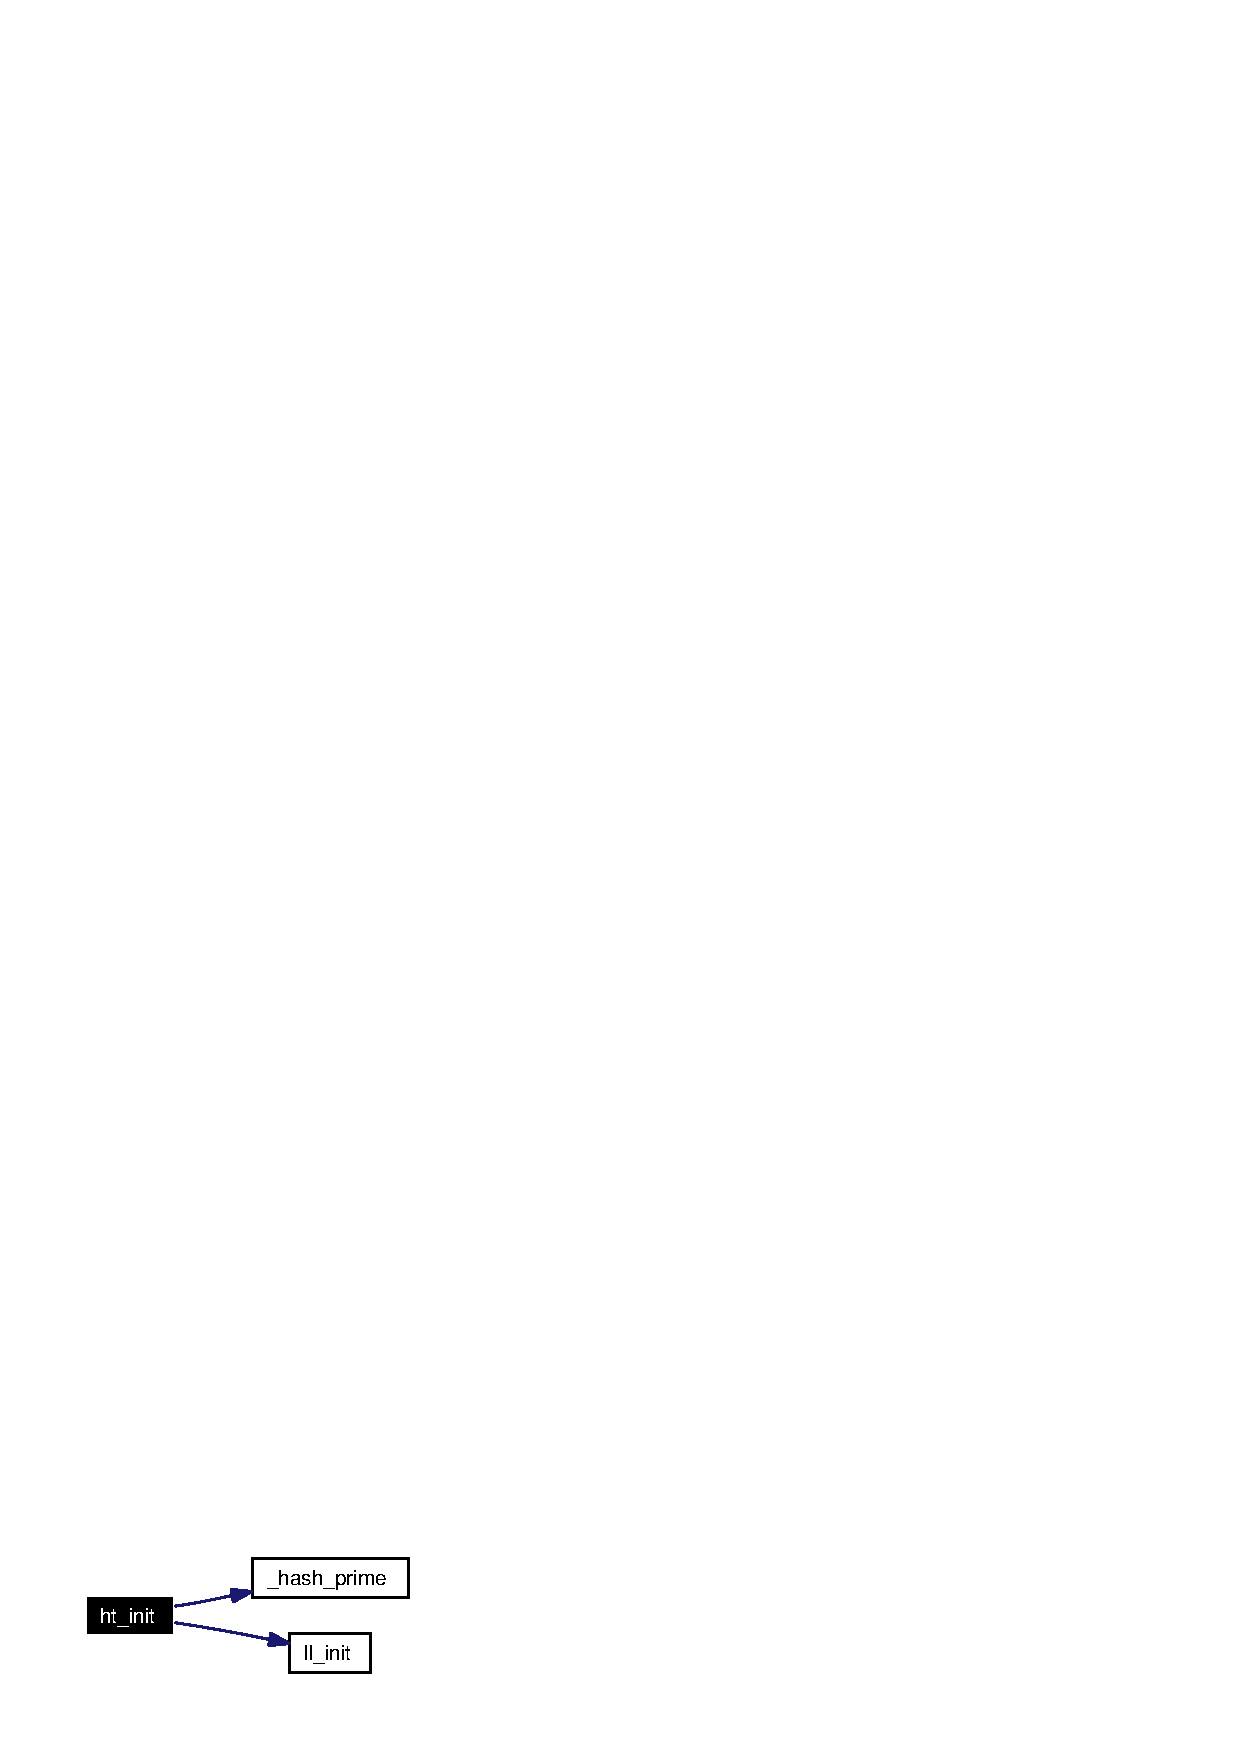
\includegraphics[width=100pt]{group__dbprim__hash_ga10_cgraph}
\end{center}
\end{figure}
\hypertarget{group__dbprim__hash_ga15}{
\index{dbprim_hash@{dbprim\_\-hash}!ht_iter@{ht\_\-iter}}
\index{ht_iter@{ht\_\-iter}!dbprim_hash@{dbprim\_\-hash}}
\subsubsection[ht\_\-iter]{\setlength{\rightskip}{0pt plus 5cm}unsigned long ht\_\-iter (\hyperlink{struct__hash__table__s}{hash\_\-table\_\-t} $\ast$ {\em table}, \hyperlink{group__dbprim__hash_ga3}{hash\_\-iter\_\-t} {\em iter\_\-func}, void $\ast$ {\em extra})}}
\label{group__dbprim__hash_ga15}


This function iterates over every entry in a hash table (in an unspecified order), executing the given {\tt iter\_\-func} on each entry.

\begin{Desc}
\item[Parameters:]
\begin{description}
\item[\mbox{$\leftarrow$} {\em table}]A pointer to a \hyperlink{group__dbprim__hash_ga1}{hash\_\-table\_\-t}. \item[\mbox{$\leftarrow$} {\em iter\_\-func}]A pointer to a callback function used to perform user-specified actions on an entry in a hash table. {\tt NULL} is an invalid value. See the documentation for \hyperlink{group__dbprim__hash_ga3}{hash\_\-iter\_\-t} for more information. \item[\mbox{$\leftarrow$} {\em extra}]A {\tt void} pointer that will be passed to {\tt iter\_\-func}.\end{description}
\end{Desc}
\begin{Desc}
\item[Return values:]
\begin{description}
\item[{\em DB\_\-ERR\_\-BADARGS}]An argument was invalid. \item[{\em DB\_\-ERR\_\-FROZEN}]The hash table is frozen.\end{description}
\end{Desc}


Definition at line 34 of file ht\_\-iter.c.

References HASH\_\-FLAG\_\-FREEZE, \_\-hash\_\-table\_\-s::ht\_\-flags, ht\_\-modulus, \_\-hash\_\-table\_\-s::ht\_\-table, ht\_\-verify, le\_\-next, le\_\-object, and ll\_\-first.

Referenced by st\_\-iter().\hypertarget{group__dbprim__hash_ga12}{
\index{dbprim_hash@{dbprim\_\-hash}!ht_move@{ht\_\-move}}
\index{ht_move@{ht\_\-move}!dbprim_hash@{dbprim\_\-hash}}
\subsubsection[ht\_\-move]{\setlength{\rightskip}{0pt plus 5cm}unsigned long ht\_\-move (\hyperlink{struct__hash__table__s}{hash\_\-table\_\-t} $\ast$ {\em table}, \hyperlink{struct__hash__entry__s}{hash\_\-entry\_\-t} $\ast$ {\em entry}, \hyperlink{struct__db__key__s}{db\_\-key\_\-t} $\ast$ {\em key})}}
\label{group__dbprim__hash_ga12}


This function moves an existing entry in the hash table to correspond to the new key.

\begin{Desc}
\item[Parameters:]
\begin{description}
\item[\mbox{$\leftarrow$} {\em table}]A pointer to a \hyperlink{group__dbprim__hash_ga1}{hash\_\-table\_\-t}. \item[\mbox{$\leftarrow$} {\em entry}]A pointer to a \hyperlink{group__dbprim__hash_ga2}{hash\_\-entry\_\-t} to be moved. It must already be in the hash table. \item[\mbox{$\leftarrow$} {\em key}]A pointer to a \hyperlink{group__dbprim_ga0}{db\_\-key\_\-t} describing the new key for the entry.\end{description}
\end{Desc}
\begin{Desc}
\item[Return values:]
\begin{description}
\item[{\em DB\_\-ERR\_\-BADARGS}]An invalid argument was given. \item[{\em DB\_\-ERR\_\-UNUSED}]Entry is not in a hash table. \item[{\em DB\_\-ERR\_\-WRONGTABLE}]Entry is not in this hash table. \item[{\em DB\_\-ERR\_\-FROZEN}]Hash table is frozen. \item[{\em DB\_\-ERR\_\-DUPLICATE}]New key is a duplicate of an existing key. \item[{\em DB\_\-ERR\_\-READDFAILED}]Unable to re-add entry to table.\end{description}
\end{Desc}


Definition at line 34 of file ht\_\-move.c.

References HASH\_\-FLAG\_\-FREEZE, \_\-hash\_\-entry\_\-s::he\_\-elem, \_\-hash\_\-entry\_\-s::he\_\-hash, \_\-hash\_\-entry\_\-s::he\_\-key, \_\-hash\_\-entry\_\-s::he\_\-table, he\_\-verify, \_\-hash\_\-table\_\-s::ht\_\-count, ht\_\-find(), \_\-hash\_\-table\_\-s::ht\_\-flags, \_\-hash\_\-table\_\-s::ht\_\-func, \_\-hash\_\-table\_\-s::ht\_\-modulus, \_\-hash\_\-table\_\-s::ht\_\-table, ht\_\-verify, LINK\_\-LOC\_\-HEAD, ll\_\-add(), and ll\_\-remove().

Here is the call graph for this function:\begin{figure}[H]
\begin{center}
\leavevmode
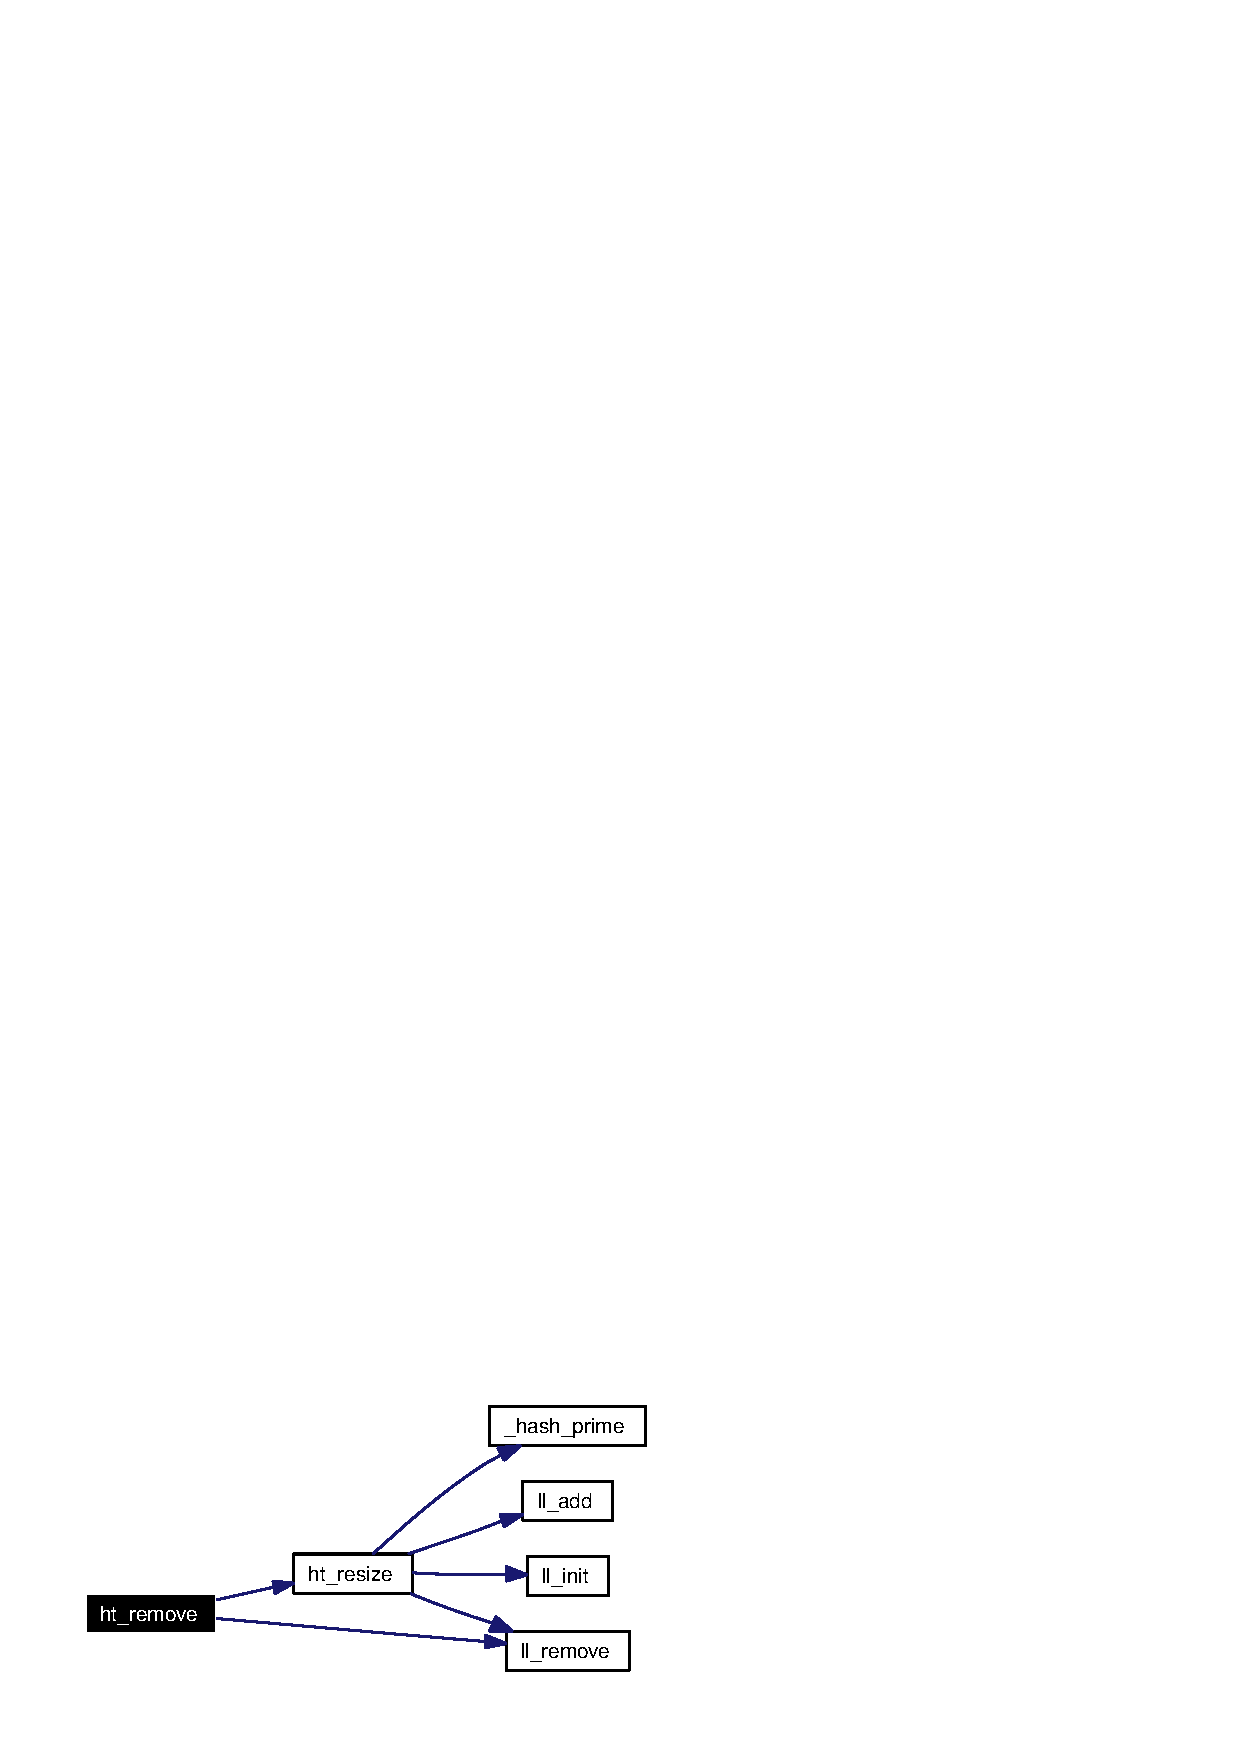
\includegraphics[width=98pt]{group__dbprim__hash_ga12_cgraph}
\end{center}
\end{figure}
\hypertarget{group__dbprim__hash_ga13}{
\index{dbprim_hash@{dbprim\_\-hash}!ht_remove@{ht\_\-remove}}
\index{ht_remove@{ht\_\-remove}!dbprim_hash@{dbprim\_\-hash}}
\subsubsection[ht\_\-remove]{\setlength{\rightskip}{0pt plus 5cm}unsigned long ht\_\-remove (\hyperlink{struct__hash__table__s}{hash\_\-table\_\-t} $\ast$ {\em table}, \hyperlink{struct__hash__entry__s}{hash\_\-entry\_\-t} $\ast$ {\em entry})}}
\label{group__dbprim__hash_ga13}


This function removes the given element from the specified hash table.

\begin{Desc}
\item[Parameters:]
\begin{description}
\item[\mbox{$\leftarrow$} {\em table}]A pointer to a \hyperlink{group__dbprim__hash_ga1}{hash\_\-table\_\-t}. \item[\mbox{$\leftarrow$} {\em entry}]A pointer to a \hyperlink{group__dbprim__hash_ga2}{hash\_\-entry\_\-t} to be removed from the table.\end{description}
\end{Desc}
\begin{Desc}
\item[Return values:]
\begin{description}
\item[{\em DB\_\-ERR\_\-BADARGS}]An invalid argument was given. \item[{\em DB\_\-ERR\_\-UNUSED}]Entry is not in a hash table. \item[{\em DB\_\-ERR\_\-WRONGTABLE}]Entry is not in this hash table. \item[{\em DB\_\-ERR\_\-FROZEN}]Hash table is frozen. \item[{\em DB\_\-ERR\_\-UNRECOVERABLE}]An unrecoverable error occurred while resizing the table.\end{description}
\end{Desc}


Definition at line 34 of file ht\_\-remove.c.

References HASH\_\-FLAG\_\-AUTOSHRINK, HASH\_\-FLAG\_\-FREEZE, \_\-hash\_\-entry\_\-s::he\_\-elem, \_\-hash\_\-entry\_\-s::he\_\-hash, \_\-hash\_\-entry\_\-s::he\_\-table, he\_\-verify, \_\-hash\_\-table\_\-s::ht\_\-count, \_\-hash\_\-table\_\-s::ht\_\-flags, ht\_\-resize(), \_\-hash\_\-table\_\-s::ht\_\-rollunder, \_\-hash\_\-table\_\-s::ht\_\-table, ht\_\-verify, and ll\_\-remove().

Referenced by \_\-st\_\-remove(), ht\_\-flush(), and st\_\-add().

Here is the call graph for this function:\begin{figure}[H]
\begin{center}
\leavevmode
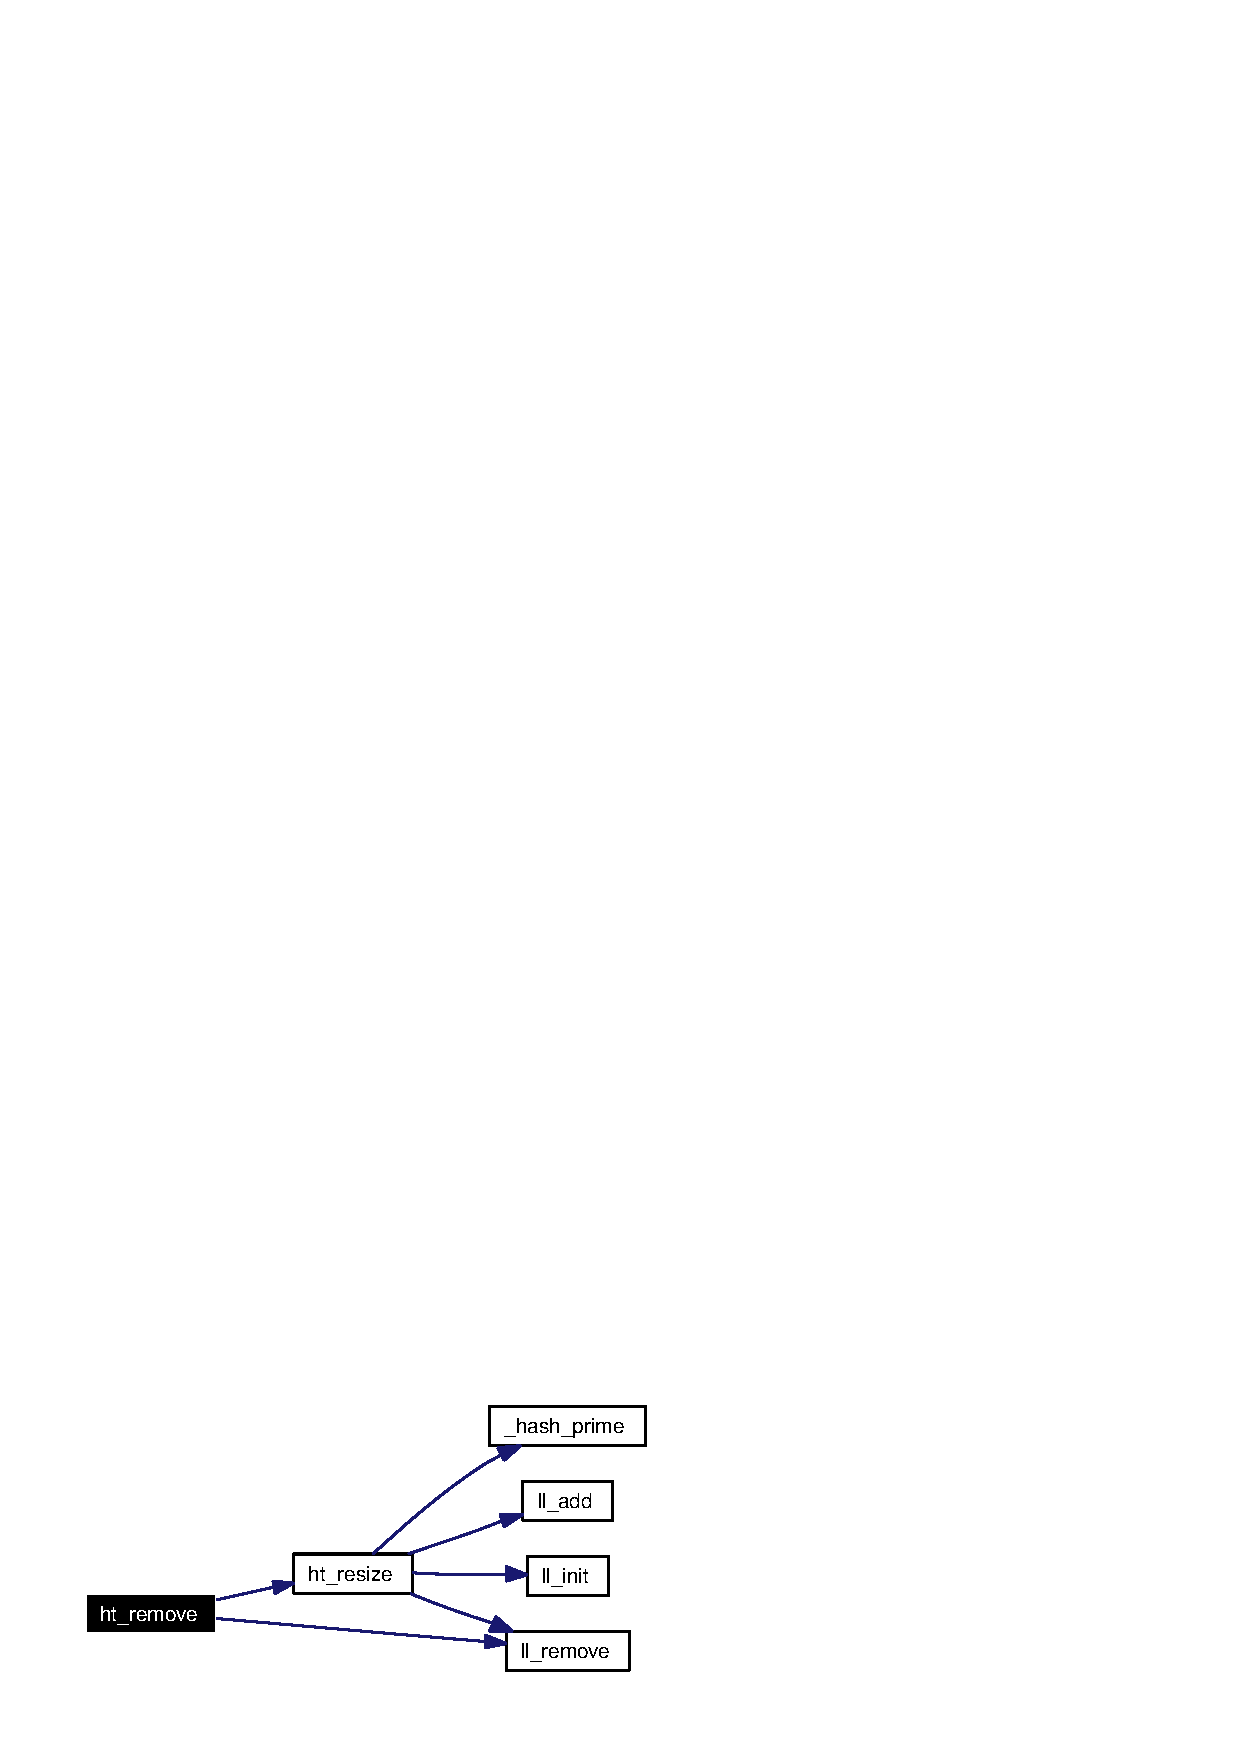
\includegraphics[width=157pt]{group__dbprim__hash_ga13_cgraph}
\end{center}
\end{figure}
\hypertarget{group__dbprim__hash_ga17}{
\index{dbprim_hash@{dbprim\_\-hash}!ht_resize@{ht\_\-resize}}
\index{ht_resize@{ht\_\-resize}!dbprim_hash@{dbprim\_\-hash}}
\subsubsection[ht\_\-resize]{\setlength{\rightskip}{0pt plus 5cm}unsigned long ht\_\-resize (\hyperlink{struct__hash__table__s}{hash\_\-table\_\-t} $\ast$ {\em table}, unsigned long {\em new\_\-size})}}
\label{group__dbprim__hash_ga17}


This function resizes a hash table to the given {\tt new\_\-size}. If {\tt new\_\-size} is 0, then an appropriate new size based on the current number of items in the hash table will be selected.

\begin{Desc}
\item[Parameters:]
\begin{description}
\item[\mbox{$\leftarrow$} {\em table}]A pointer to a \hyperlink{group__dbprim__hash_ga1}{hash\_\-table\_\-t}. \item[\mbox{$\leftarrow$} {\em new\_\-size}]A new size value for the table.\end{description}
\end{Desc}
\begin{Desc}
\item[Return values:]
\begin{description}
\item[{\em DB\_\-ERR\_\-BADARGS}]An argument was invalid. \item[{\em DB\_\-ERR\_\-FROZEN}]The table is currently frozen. \item[{\em DB\_\-ERR\_\-UNRECOVERABLE}]A catastrophic error was encountered. The table is now unusable. \item[{\em ENOMEM}]No memory could be allocated for the new bucket table.\end{description}
\end{Desc}


Definition at line 38 of file ht\_\-resize.c.

References \_\-hash\_\-fuzz, \_\-hash\_\-prime(), \_\-hash\_\-rollover, \_\-hash\_\-rollunder, HASH\_\-FLAG\_\-FREEZE, \_\-hash\_\-entry\_\-s::he\_\-hash, \_\-hash\_\-entry\_\-s::he\_\-key, \_\-hash\_\-table\_\-s::ht\_\-count, \_\-hash\_\-table\_\-s::ht\_\-flags, \_\-hash\_\-table\_\-s::ht\_\-func, ht\_\-modulus, \_\-hash\_\-table\_\-s::ht\_\-modulus, \_\-hash\_\-table\_\-s::ht\_\-resize, \_\-hash\_\-table\_\-s::ht\_\-rollover, \_\-hash\_\-table\_\-s::ht\_\-rollunder, \_\-hash\_\-table\_\-s::ht\_\-table, ht\_\-verify, le\_\-object, LINK\_\-LOC\_\-HEAD, ll\_\-add(), ll\_\-first, ll\_\-init(), and ll\_\-remove().

Referenced by ht\_\-add(), ht\_\-remove(), and st\_\-resize().

Here is the call graph for this function:\begin{figure}[H]
\begin{center}
\leavevmode
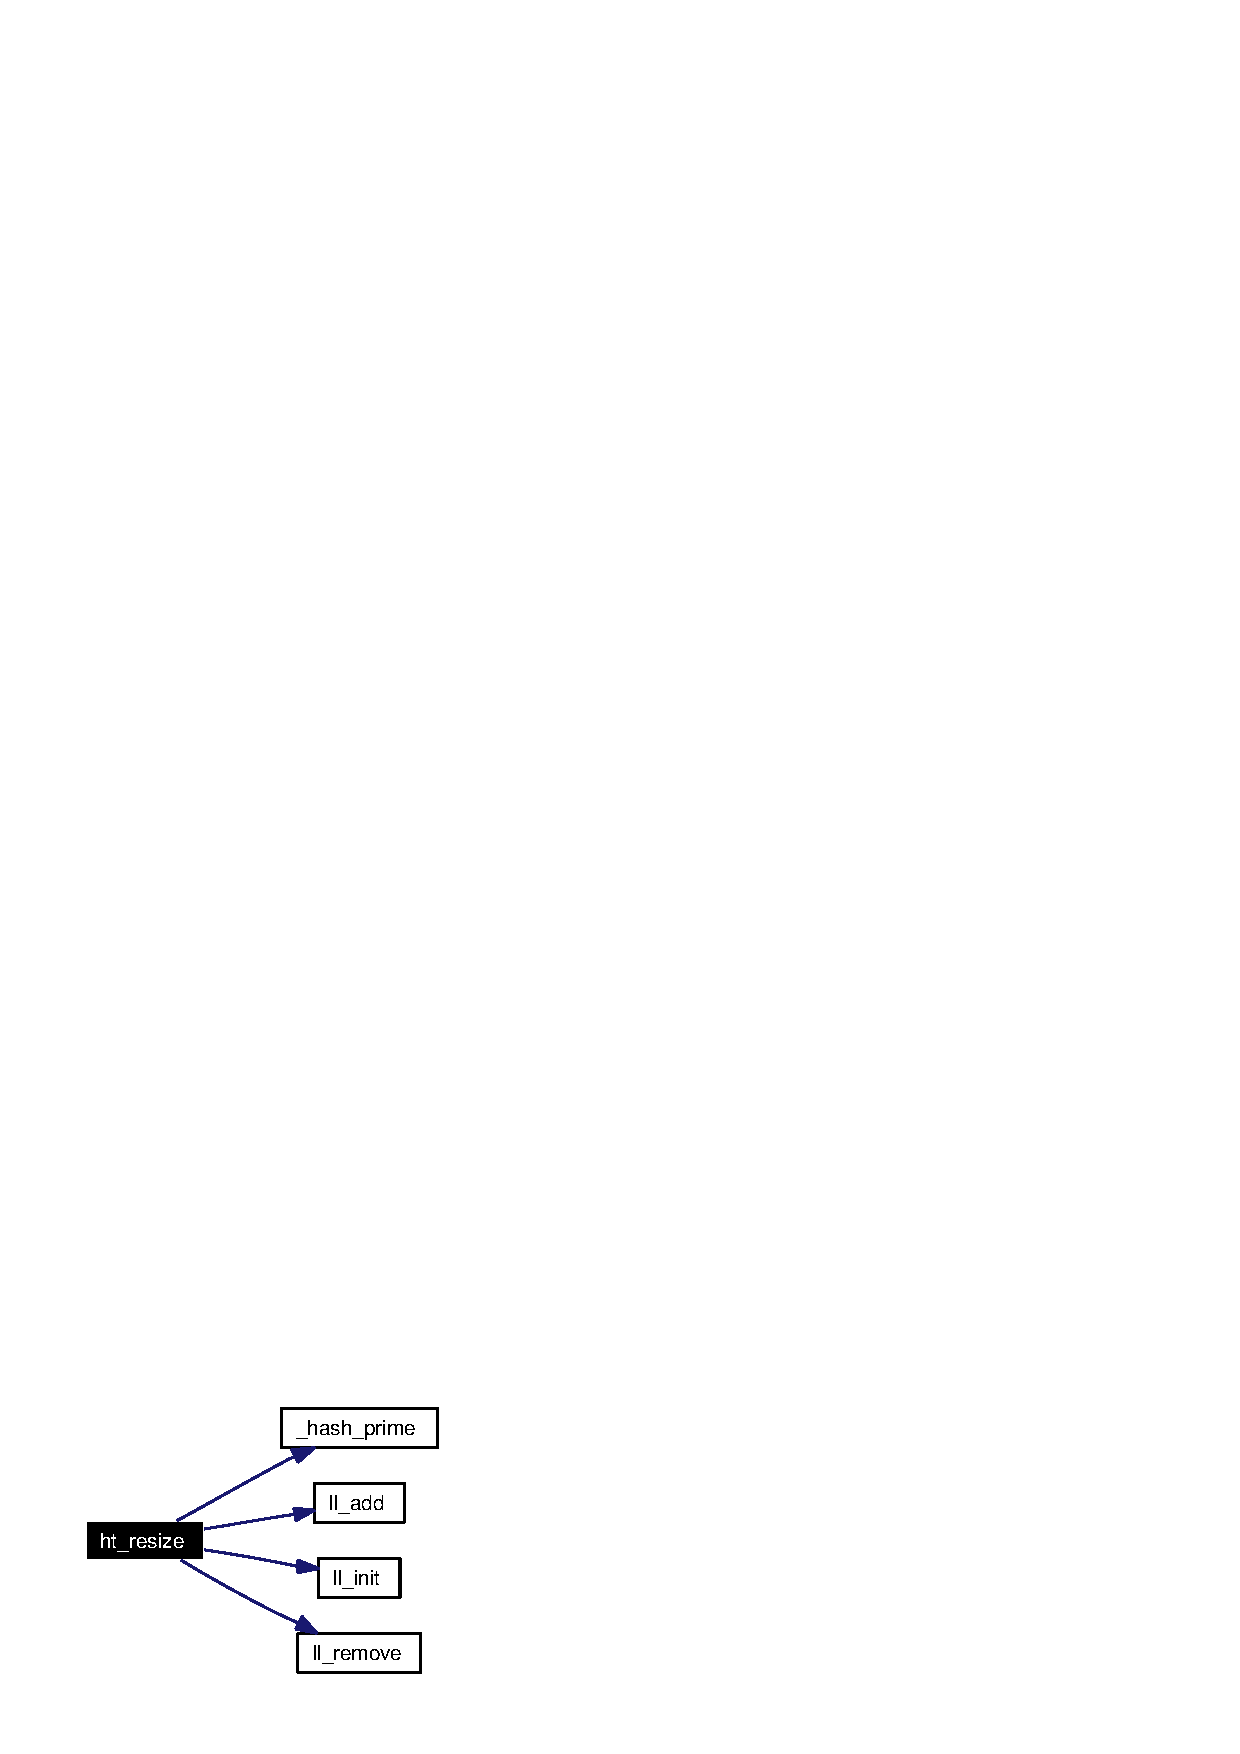
\includegraphics[width=107pt]{group__dbprim__hash_ga17_cgraph}
\end{center}
\end{figure}


\subsection{Variable Documentation}
\hypertarget{group__dbprim__hash_ga0}{
\index{dbprim_hash@{dbprim\_\-hash}!primes@{primes}}
\index{primes@{primes}!dbprim_hash@{dbprim\_\-hash}}
\subsubsection[primes]{\setlength{\rightskip}{0pt plus 5cm}unsigned long \hyperlink{group__dbprim__hash_ga0}{primes}\mbox{[}$\,$\mbox{]}\hspace{0.3cm}{\tt  \mbox{[}static\mbox{]}}}}
\label{group__dbprim__hash_ga0}


\begin{Desc}
\item[For internal use only.]
This variable contains a table of 16-bit prime numbers, used by \hyperlink{group__dbprim__hash_ga20}{\_\-hash\_\-prime()} to test the primality of potential primes.\end{Desc}


Definition at line 50 of file \_\-hash\_\-prime.c.

Referenced by \_\-hash\_\-prime().